\documentclass[twoside,11pt]{article}

% Any additional packages needed should be included after jmlr2e.
% Note that jmlr2e.sty includes epsfig, amssymb, natbib and graphicx,
% and defines many common macros, such as 'proof' and 'example'.
%
% It also sets the bibliographystyle to plainnat; for more information on
% natbib citation styles, see the natbib documentation, a copy of which
% is archived at http://www.jmlr.org/format/natbib.pdf

\usepackage{jmlr2e}
\usepackage{amsmath,amssymb}
\usepackage{algorithm}
\usepackage{algorithmic}
\usepackage{verbatim}
\usepackage{wrapfig}
\usepackage{color}
\usepackage{stfloats}
\usepackage{float}
\usepackage{natbib}
\setlength{\bibsep}{7pt}



% Definitions of handy macros can go here

\newcommand{\dataset}{{\cal D}}
\newcommand{\fracpartial}[2]{\frac{\partial #1}{\partial  #2}}
\newcommand{\fix}{\marginpar{FIX}}
\newcommand{\new}{\marginpar{NEW}}

\newcommand{\argmax}{\operatornamewithlimits{argmax}}
\newcommand{\argmin}{\operatornamewithlimits{argmin}}
\newcommand{\x}{\mathbf{x}}
\newcommand{\e}{\mathbf{e}}
\newcommand{\cc}{\mathbf{c}}
\newcommand{\w}{\mathbf{w}}
\newcommand{\z}{\mathbf{z}}
\newcommand{\rr}{\mathbf{r}}
\newcommand{\q}{\mathbf{q}}
\newcommand{\bb}{\mathbf{b}}
\newcommand{\hl}{\mathbf{h}}
\newcommand{\dl}{\boldsymbol{\delta}}
\newcommand{\ab}{\boldsymbol\alpha}
\newcommand{\bl}{\boldsymbol{\beta}}
\newcommand{\bp}{\boldsymbol{\phi}}
\newcommand{\btheta}{\boldsymbol{\theta}}
\newcommand{\y}{\mathbf{y}}
\newcommand{\Lb}{\mathbf{L}}
\newcommand{\Wb}{\mathbf{W}}
\newcommand{\Ib}{\mathbf{I}}
\newcommand{\Kb}{\mathbf{K}}
\newcommand{\Hb}{\mathbf{H}}
\newcommand{\Qb}{\mathbf{Q}}
\newcommand{\Pb}{\mathbf{P}}
\newcommand{\Xb}{\mathbf{X}}
\newcommand{\Sb}{\mathbf{S}}
\newcommand{\Rb}{\mathbf{R}}
\newcommand{\Fb}{\mathbf{F}}
\newcommand{\fullname}{Gradient Boosted Feature Extraction}
\newcommand{\name}{GBFE}
\newcommand{\eddie}{\textcolor{black}}
\newcommand{\kilian}{\textcolor{red}}
\definecolor{orange}{rgb}{1,0.5,0}
\newcommand{\Matt}{\textcolor{green}}
%\newcommand{\Matt}{\textcolor{black}}
\newcommand{\oc}[1]{\textbf{[OC: #1]}}
\sloppy


% Heading arguments are {volume}{year}{pages}{submitted}{published}{author-full-names}

\jmlrheading{1}{2012}{1-48}{4/00}{10/00}{Zhixiang (Eddie) Xu, Matt J. Kusner, Gao Huang, Kilian Q. Weinberger, Alice X. Zheng, Olivier Chapelle}

% Short headings should be running head and authors last names

\ShortHeadings{Feature Extraction with Gradient Boosted Regression Trees}{Xu, Kusner, Huang, Zheng, and Chapelle}
\firstpageno{1}

\begin{document}

\title{Feature Extraction with Gradient Boosted Regression Trees}

\author{\name Zhixiang (Eddie) Xu \email xuzx@cse.wustl.edu \\
       \addr Citadel\\
       Chicago, IL 60603, USA\\
       % \addr Department of Computer Science\\
       % Washington University\\
       % St. Louis, MO 63130, USA
       \AND
       \name Matt J.\ Kusner \email mkusner@wustl.edu \\
       \addr Department of Computer Science\\
       Washington University\\
       St. Louis, MO 63130, USA\\
       % \addr Department of Computer Science\\
       % Washington University\\
       % St. Louis, MO 63130, USA
       \AND
       \name Gao Huang \email g09@mails.tsinghua.edu.cn
       \AND
       \name Kilian Q.\ Weinberger \email kilian@wustl.edu \\
       \addr Department of Computer Science\\
       Cornell University\\
       Ithaca, NY 14853, USA\\
       \AND
       \name Alice X.\ Zheng \email alicez@graphlab.com \\
       \addr GraphLab\\
       Seattle, WA 98051, USA
	   \AND
       \name Olivier Chapelle \email olivier@chapelle.cc \\
       \addr Criteo\\
       Palo Alto, CA 94301, USA}	   
	   
	   


\editor{XXX}

\maketitle

\begin{abstract}%   <- trailing '%' for backward compatibility of .sty file
%!TEX root=gm_jmlr.tex 

Gradient Boosted Regression Tree (GBRT) algorithms have been widely used in many real-world applications such as web-search ranking, image detection and budgeted learning. This is largely due to its robustness to noisy data, non-linear feature combinations and fast evaluation speed. However, very few prior works focus on applying GBRT to feature extraction. One key observation is that certain 
%Some 
unique properties of GBRT, such as non-continuous boosted functions and optimization in function space, make GBRT well-suited for feature extraction. In this paper, we develop a novel algorithm called \fullname{} (\name{}), that leverages the unique properties of GBRT for feature extraction in two settings: budgeted learning and feature selection. 
%We give insights of unique properties of GBRT boosted functions, and derive our algorithm for test-time budgeted learning and non-linear feature selection. 
As part of the derivation, we give insights of unique properties of GBRT boosted functions that may be of independent interest. We further develop a simple method to estimate the lower bound of the prediction variance given extracted features using \name{}. We evaluate our algorithm on several real-world data sets for budgeted learning and feature selection, and demonstrate that \name{} outperforms the current state-of-the-art.
\end{abstract}

\begin{keywords}
  Feature Extraction, Budgeted Learning, Gradient Boosting, Regression Trees
\end{keywords}

\section{Introduction}
%!TEX root=gm_jmlr.tex 

Gradient Boosted Regression Trees (GBRT) \citep{friedman2001greedy} are widely used in many real-world applications. GBRT non-linearly partitions the input space using decision trees, and thus is readily suited for learning tasks with unbalanced and complex data. For instance, in a recent web-search ranking competition, eight winners of two competition tracks all use ensemble based decision tree algorithms \citep{chapelle2011yahoo}. In the meantime, compared to other classifiers, its unique functional optimization procedure makes feature extraction very easy. It separates feature extraction and classifier optimization into two separate stages, and thus structured feature information can be seamlessly incorporated. Moreover, its evaluation time is linear w.r.t. the number of testing inputs, and this makes GBRT very scalable to large feature extraction problems.

Feature extraction plays a crucial role %recently been revisited 
in two popular learning scenarios: budgeted learning \citep{xu2014classifier} and feature selection \citep{guyon2003introduction}. In the budgeted learning setting, researchers focus on reducing the computational costs (and potentially other related costs) of classification during test-time. This test-time computational cost often consists of two components: (a) the running time of the algorithm and (b) the time required for extracting features used by the algorithm. In this work, we focus on the scenario where the feature extraction cost is dominant. Imagine introducing a new feature to an algorithm that is executed one million times per day which improves the accuracy by 1\%, but also increases the extraction time by 1$s$ per execution. %and this algorithm is executed a million times per day. 
This new feature would require allocating 5 days of additional CPU time every day. Such scenarios are commonplace in large-scale web-search ranking \citep{zheng2007general} and email spam filtering \citep{weinberger2009feature}. Therefore feature extraction must be strictly accounted for. 

In the feature selection setting, researchers are concerned with how a classifier can predict a label and the features it uses. As the size of data sets grow, % increasingly larger and larger, 
a good feature selection algorithm should not only be able to identify relevant features, but also be scalable to large amount of training inputs. Additionally, in various applications such as bio-informatics~\citep{saeys2007review}, information about inter-feature dependency should also be considered during feature selection. In both budgeted learning and feature selection, efficiently extracting features for a very large data set plays a key role in designing a learning algorithm.

In this paper, we introduce a new algorithm: \fullname{} (\name{}) that is designed for efficient feature extraction in a large scale setting. \name{} is based on Gradient Boosted Regression Trees (GBRT), and therefore inherits many desirable properties that are suitable for feature extraction. Firstly, \name{} retains the capabilities of coping with non-linear interactions between features and labels from GBRT, and thus can discover non-linear dependencies. Secondly, unlike other feature extraction algorithms used in budgeted learning or feature selection, which use computationally-expensive kernel methods~\citep{scholkopf2001learning} or complex cascade structures \citep{cambazoglu2010early,chen2011,Saberian2010,Lefakis2010}, \name{} maintains non-linearity very efficiently, and thus scales to large data sets %containing a large number of samples 
while it is simultaneously %and is 
very easy to implement and use. Thirdly, due to the unique two-step functional optimization procedure %two steps function space optimization 
of GBRT, \name{} can easily handle side information about structured feature dependency. This structured feature dependency is commonly seen in applications such as bio-informatics \citep{saeys2007review} %feature selection and budgeted learning for 
and computer vision \citep{felzenszwalb2010object}. Finally, \name{} unifies feature extraction and classification into one optimization problem, pushing the feature extraction into the classifier learning. 

Two earlier short papers already introduce \name{} in two different settings, Greedy Miser~\citep{greedymiser} for budgeted learning and Gradient Boosted Feature Selection (GBFS)~\citep{xu2014gradient} for feature selection. However, this manuscript provides significantly more insight, discussion, and experimental results than prior work. The paper is organized as follows. In Section \ref{sec:background} we first define the notation used in the paper and describe some background knowledge. We then investigate the unique properties of GBRT and give insights why its two-step optimization is useful for feature extraction in Section~\ref{sec:gbrt}. In Section~\ref{sec:greedymiser}, we introduce and define the test-time budgeted learning setting. We then construct an optimization problem for test-time budgeted learning and derive our algorithm for budgeted learning (\name{}-BL) by solving the optimization problem. In Section \ref{sec:gbfs} we connect budgeted learning and feature selection, and introduce a variant of \name{} tailored for efficient feature selection (\name{}-FS). In Section \ref{sec:variance}, we introduce a simple analysis method for bounding the prediction variance of \name{}. In Section \ref{sec:results} we demonstrate the performance of our algorithm on several real-world benchmark data sets for budgeted learning and feature selection, and also discuss using the prediction variance analysis as a convergence tool. Section \ref{sec:related} reviews the prior and related work that inspires our paper. Finally, in Section \ref{sec:conclusion}, we conclude and propose several potential future approaches.





\section{Notation and Background}
\label{sec:background}
%!TEX root=gm_jmlr.tex 
In this section, we define our notation and introduce some related background algorithms.
Our data consist of $n$ input vectors {$\{\x_1, \ldots, \x_n\}\! \in\! {\cal R}^p$} with corresponding labels $\{y_1, \ldots, y_n\}\!\in\!{\cal Y}$ drawn from an unknown joint distribution ${\cal D}$. Labels can be continuous (regression) or categorial (binary or multi-class classification). In this paper, we focus on feature extraction for large-scale data sets, and thus we assume that the number of inputs is much larger than the number of features ($n \gg p$). %MATT%: algorithms work for either case yeah (i.e., p >> n)? might be worth advertising both cases
%%%We also assume that each feature $\alpha$ has an acquisition cost $c_{\alpha}\! >\! 0$ during its initial retrieval. Since feature value can be cached efficiently, all subsequent retrieval on this feature is free. (maybe move into Section 4)

\subsection{The capped $l_1$-norm}
The $l_1$-norm is often used to regularize a classifier to avoid over-fitting. It is a so-called `shrinkage' operator \citep{tibshirani1996regression} in that it `shrinks' coefficients towards $0$, making the resulting solution sparse. As such, the $l_1$-norm is a popular choice in feature selection models. However, the effect of shrinkage is to reduce the magnitude of all coefficients \emph{regardless of feature quality}. To remedy this, 
%, and it also makes the solution sparse. However, these two effects are tied to each other, enforcing sparsity will also reduce the complexity of the classifier. 
\citet{zhang2009multi} introduces the \emph{capped} $l_1$-norm, which is defined by the element-wise operation:
\begin{align}
	\|\beta_j\|_{\lceil 1} = \min(|\beta_j|,\epsilon). \label{eq:cappedl1}
\end{align}
The capped $l_1$-norm is show in Figure~\ref{fig:cappedl1}. It behaves like the regular $l_1$-norm when $|\bl|$ is small, but is capped to a constant $\epsilon$ when $|\bl| \ge \epsilon$. Similar to the $l_0$-norm, the capped $l_1$-norm does not penalize large coefficients. In other words, once a feature $j$ is extracted, (i.e., $|\beta_j| > 0$) its subsequent use is not penalized as its value increases beyond $\epsilon$. When $\epsilon$ is small enough (\emph{i.e. }$\epsilon \le \min_p|\beta_j|$), the exact number of features extracted can be computed with $\frac{q_\epsilon(\bl)}{\epsilon}$. \Matt{What's $q_\epsilon$ here? I'm not exactly sure}
\begin{figure*}[t!!!]
\centerline{
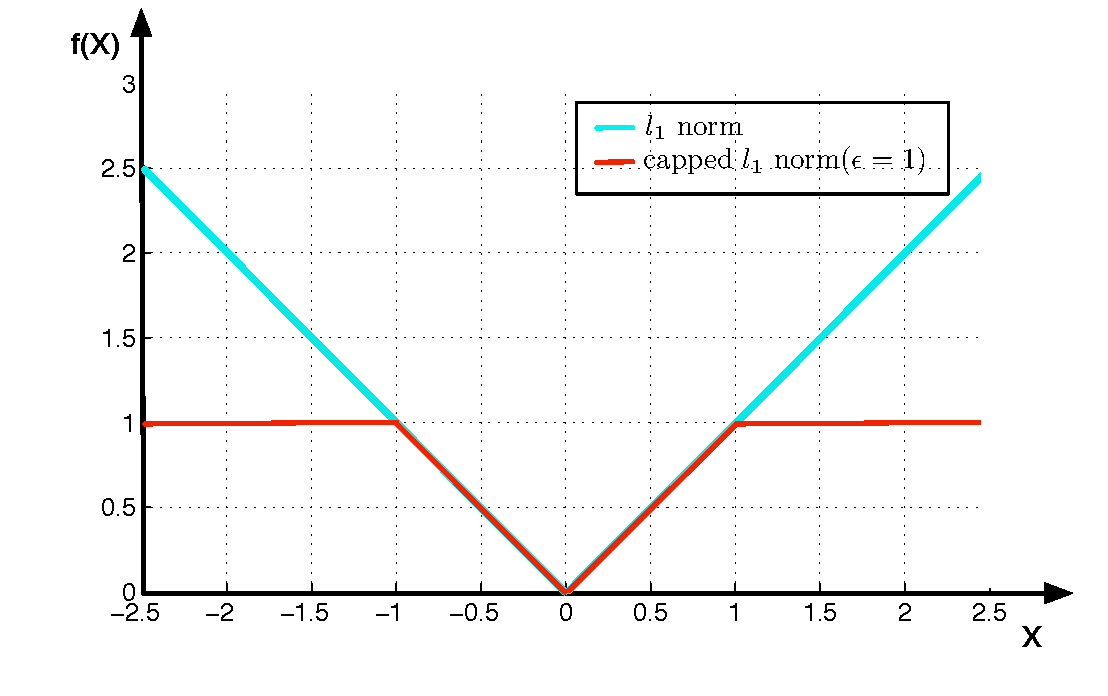
\includegraphics[width = 0.5\textwidth]{plots/cappedl1.pdf}%{plots/simul_iter}
}
\caption{The capped $l_1$-norm. It behaves like the regular $l_1$-norm when $|\bl|$ is small, but is capped to a constant $\epsilon$ when $|\bl| \ge \epsilon$.}
\label{fig:cappedl1}
\end{figure*}

\subsection{Predicting Function} We model the mapping from features to labels using a predicting function $H : {\cal R}^p \rightarrow {\cal Y}$. We learn this function by minimizing a loss function $\ell(H)$,
\begin{align}
	\min_H \ell(H). \label{eq:loss}
\end{align}
The loss function can be squared-loss for regression,
\begin{align}
	\ell_{sq}(H) = \frac{1}{n}\sum_{i=1}^n (H(\x_i) - y_i)^2, \label{eq:sqrloss}
\end{align}
or other losses such as the logistic loss for classification.

\subsection{Gradient Boosted Regression Trees (GBRT)} 
\label{sec:bg_gbrt}
Gradient Boosted Regression Trees (GBRT)~\citep{friedman2001greedy} learns the predicting function $H$ by optimizing a loss function such as (\ref{eq:sqrloss}) using gradient boosting. The learned predicting function is an additive classifier consisting of weak learners, 
\begin{align}
	H(\x) = \sum_t h_t(\x) \beta_t, \label{eq:H}
\end{align}
where $\beta_t$ is the learning rate and $h_t(\cdot)$ is a weak learner. Each weak learner $h_t \in {\cal H}$ is a regression tree \citep{breiman1984classification}, and ${\cal H}$ is the set of all possible regression trees of some limited depth $b$. At each iteration $t + 1$, a new weak learner (regression tree) is generated to minimize the loss function $\ell$. This is achieved by building a non-linear regression tree to approximate the negative gradient of $\ell$ w.r.t. current predicting function $H^t$,
\begin{align}
	h_{t+1} = \argmin_{h_{t+1}} \sum_i \Big( - \frac{\partial \ell}{\partial H^t(\x_i)} - h_{t+1}(\x_i)\Big)^2. \label{eq:CART}
\end{align}
The greedy Classification and Regression Tree (CART) algorithm \citep{breiman1984classification} is usually used to generate such a tree. Specifically, CART builds a limited depth regression tree $h_t \in {\cal H}$ by greedily minimizing an impurity function, which could be a squared loss as in (\ref{eq:CART}) for regression problems or an entropy loss for classification problems. Since in GBRT, the negative gradients $-\frac{\partial \ell}{\partial H^t(\x_i)}$ are real numbers, CART is run to minimize the squared impurity loss function (\ref{eq:CART}). It minimizes the loss function by repeatedly splitting the data on a feature per tree-node. Since CART recursively splits data using different features, it can non-linearly combine features.

From eq.(\ref{eq:H}), we see that $H$ is simply a linear function of weak learners parameterized by coefficient $\bl$, 
\begin{align}
H(\x) = \hl(\x)^\top\bl, \textrm{ where }\hl(\x) = [h_1(\x),\dots,h_T(\x)]^\top. \label{eq:boosting-trick}
\end{align}
%Each $h_t(\x) \in {\cal H}$ is a limited depth regression tree. Since ${\cal H}$ contains all possible regression trees of some limited depth, and its size $|{\cal H}| = T$ is very large, the coefficient $\bl$ is usually very sparse. This indicates that the classifier $H$ only uses a relatively small amount of trees.
%\Matt{I omitted the previous 3 sentences here} 
Imagine $h_1(\x),\dots,h_T(\x)$ is the set of all possible hypotheses in ${\cal H}$ so that $T = |{\cal H}|$. We can thus interpret the function $h(\cdot)$ as a non-linear transformation of the feature space by ${\cal H}$ as such, $\x \rightarrow \hl(\x)$, which is called the `boosting trick' \citep{friedman2001greedy,chapelle2011boosted,rosset2004boosting}. Since regression trees are negation closed (\emph{i.e.} $\forall h \in {\cal H}, \exists -h \in {\cal H}$), we assume the coefficients $\bl \ge 0$ without loss of generality. 

Finally, we define a binary indicator matrix $\Fb \in \{0,1\}^{p \times T}$. An entry in $F_{\alpha t} = 1$ if and only if feature $\alpha$ is used somewhere to split the regression tree $t$.

\section{Unique Properties of Gradient Boosted Regression Trees}
\label{sec:gbrt}
%!TEX root=gm_jmlr.tex
In this section, we analyze Gradient Boosted Regression Trees (GBRT) in detail and give insights of unique properties of GBRT. We compare GBRT with a linear classifier and a kernel classifier. Let $\theta$ denote the parameters of a classifier $H$. The goal of learning a classifier is to learn these parameters $\theta$ by minimizing a loss function $\ell$. These parameters are usually learned by gradient descent, where at each iteration, we compute the gradient of the loss function $\ell$ w.r.t. parameters, $\frac{\partial \ell}{\partial \theta}$. We apply the generalized chain rule, and decompose this gradient into two parts:
\begin{align}
	\frac{\partial \ell}{\partial \theta} = \sum_{i=1}^n \frac{\partial \ell}{\partial H(\x_i)} \frac{\partial H(\x_i)}{\partial \theta}, \label{eq:chainrule}
\end{align}  
where $H(\x_i)$ is the prediction of input $\x_i$. Note that the first part $\frac{\partial \ell}{\partial H(\x_i)}$ is the gradient of the loss function $\ell$ w.r.t. predicting function in the function space evaluated at an input $\x_i$, and the second part is the gradient of the predicting function w.r.t. its parameter $\theta$. Compared to linear classifiers and kernel classifiers, there are two unique properties of GBRT: implicit parameterization and non-linear feature combination.

\subsection{Implicit parameterization} Both linear classifier and kernel classifier have a predicting function $H$ that can be represented as an analytical function of its parameters (\emph{i.e.} for linear classifier, $H(\x) = \x^\top\theta$, where $\theta \in {\cal R}^p$). Therefore, when optimizing a linear or a kernel classifier, one usually optimizes the classifier parameters directly through the gradient of the loss w.r.t. classifier parameters (\emph{i.e. }$\frac{\partial \ell}{\partial \theta}$). In contrast, there is no such an \emph{analytical} function to model the predicting function $H$ in GBRT, and one has to learn the parameters of the GBRT predicting function in two steps. In other words, GBRT is parameterized implicitly. First, GBRT computes the gradient of the loss function w.r.t. the predicting function $H$ in function space $\frac{\partial \ell}{\partial H(\x_i)}$ evaluated at each input sample $\x_i$. Second, GBRT approximates this functional gradient $\frac{\partial \ell}{\partial H(\x_i)}$ at every input $\x_i$ by building a limited depth regression tree $h(\cdot)$ using the CART algorithm, which minimizes a squared impurity function (\ref{eq:CART}). Note that features are only used when approximating the negative gradient during the second step, and therefore we can add constraints for feature extraction here. This two-step optimization procedure provides more flexibility to incorporate structured feature information commonly used in bio-informatics and computer vision. However, these two steps are also very closely connected, and we will show their connections in Section~\ref{sec:greedymiser}. 

\subsection{Nonlinear feature combination} Different from linear classifiers, GBRT is capable of approximating a non-linear gradient surface. Figure~\ref{fig:simul} (plot (a)), shows a scenario where sample inputs are not linearly-separable. Plots (b)-(d) show the functional gradient surface $\frac{\partial \ell}{\partial H}$ of each classifier. GBRT approximates the gradient surface through limited depth regression trees. For a depth $3$ tree, which has $2^{3-1} = 4$ leaf nodes, GBRT essentially approximates the gradient surface by partitioning the space into 4 blocks (shown in plot (d)). In contrast, a linear gradient is just a hyperplane in the input space (\emph{i.e. } $\x^\top (\frac{\partial \ell}{\partial \theta})$), which is shown in plot (b). Kernel classifiers can achieve non-linear gradients through the kernel-trick, shown in plot (c). However, the key advantage of GBRT is that it achieves this non-linearity in a parametric way. For a depth $3$ tree, its parameters are only $3$ features and corresponding splitting values. In contrast, kernel methods achieves non-linearity through a non-parametric kernel that depend on the size of the data. During test-time, parametric GBRT is much faster than non-parametric methods and therefore is very suitable for large scale data sets and test-time cost-sensitive applications. 
 
\begin{figure*}[t!!!]
\centerline{
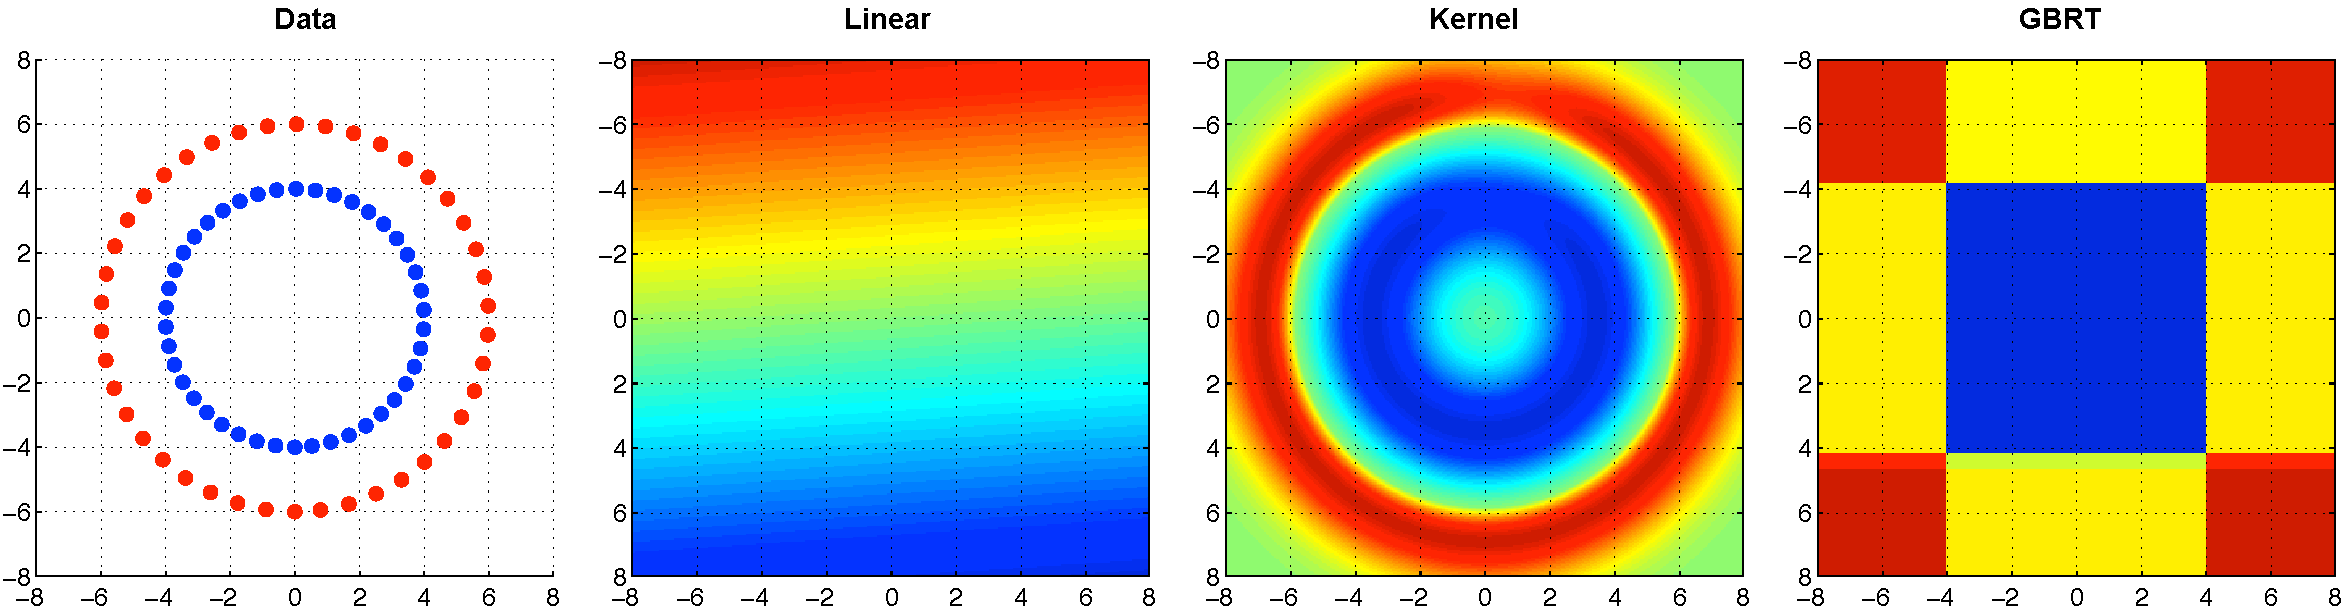
\includegraphics[width = \textwidth]{plots/grad_simul.pdf}%{plots/simul_iter}
}
\caption{Gradient surface of linear, kernel and GBRT classifiers. (a) The linearly-unseparable simulation data. Red dots and blue dots are from two different classes, and the task is binary classification. (b) The gradient surface of a linear classifier, which is a hyperplane (c) The gradient surface of a kernel classifier. Kernel methods achieve non-linear gradient surfaces in a non-parametric way. (d) The gradient surface of a GBRT classifier. }
\label{fig:simul}
\end{figure*}





% \textbf{Implicit parameterization.}
% However, the first key difference between GBRT and classifiers that are commonly combined with manifold regularization (e.g., linear and kernelized logistic regression, support vector machines, least squares regression) is that the predicting function $H(\cdot)$ of GBRT \emph{is not explicitly parameterized}. Specifically, $H(\cdot)$ is not an analytical function of its parameters
%  (i.e. decision tree splitting features and corresponding splitting values). Therefore, we cannot compute the gradient $\frac{\partial H(\x_i)}{\partial \theta}$. In contrast, the majority of other classifiers have predicting functions that can be represented as an analytic function of its parameters,
%  and the gradient in eq.~(\ref{eq:chain_gradient}) can be computed normally. Without an explicit parameterization for $H(\cdot)$, gradient boosting requires a function to approximately match the functional gradient $g(\cdot) = \frac{\partial {\cal L}}{\partial H(\cdot)}$ \emph{directly}.
%
%
% \textbf{Discontinuous gradient approximation.}
% GBRT approximates the functional gradient $g(\x)$ at every input $\x$ using a limited depth regression tree $h(\x)$, as shown in eq.~(\ref{eq:cart}). Note that a depth $d$ tree makes at most $2^{d-1}$ different predictions. Therefore, this approximation is discontinuous wherever the regression tree splits on a feature. Because this approximation is done using regression trees, \emph{the similarity of functional gradients for nearby inputs is not guaranteed}. We demonstrate this difficulty on a synthetic binary classification dataset.
%
% Figure~\ref{fig:illu} depicts a simple one-dimensional dataset with two known labels. We plot the predictions passed through link function $\sigma(\cdot)$ that we obtained from GBRT with manifold regularization after different numbers of iterations. In each plot, the vertical black lines indicate the regression tree at the current iteration split the data. We initialize the predicting function to be $H^0(\x_i) = H^0(\bar{\x}_j) = 0; \forall i,j$ (as we have no prior for the labels of unlabeled inputs), and thus all inputs have link value $\sigma(H^0(\x)) = 0.5$. At the first iteration, because all inputs have the same prediction, only labeled inputs (the first and last) have non-zero gradient (from the loss $\ell(\cdot)$). Thus, GBRT learns a regression tree to predict the first input closer to 1 and the last input closer to 0, while keeping the predictions of unlabeled inputs unchanged. The second iteration again only the predictions of the first and last inputs change. At the fifth iteration the dataset is still largely unchanged save a few inputs neighboring the first and last inputs. Even after 100 iterations roughly one third of the dataset has predictions identical to their initial predictions. Finally, after 500 iterations the dataset is clearly separated. In effect, GBRT with manifold regularization will require a large number of trees, even for simple datasets, to propagate gradients of labeled inputs to nearby unlabeled inputs. We refer to this problem as  \emph{gradient propagation delay}.
%







\section{Budgeted Learning}
\label{sec:greedymiser}
%!TEX root=gm_jmlr.tex 
In this section, we first describe the test-time budgeted learning setting, and then introduce our Gradient Boosted Feature Extraction algorithm variant for budgeted learning. As described in~(\ref{eq:boosting-trick}), the classifier $H$ can be regarded as a linear function of weak learners $h_1, \ldots, h_T$, %\hl$
parameterized by coefficients $\bl$. As costs will arise from weak learners $h_t$, we will formalize the test-time computational cost of evaluating the classifier $H$ as a function of the sparsity of a given weight-vector $\bl$ (indicating whether each $h_t$ is used or not). 

\subsection{Test-time computational cost}
The test-time computational cost of $H$ consists of two parts: (a) the evaluation cost of all trees $h_t$ with $\bl_t > 0$ and (b) the extraction cost of features used in these trees. Let $c_e$ denote the single tree evaluation cost, and $c_\alpha$ the cost of extracting feature $\alpha$ the first time (since feature values can be cached efficiently, all subsequent retrieval on this feature is free). Note that $c_e$ is a constant independent of the number of training sample inputs, and is usually very small if the tree depth is small. Thus, the fact that GBRT is a parametric classifier is an key advantage of GBRT over other non-linear algorithms (e.g., kernel-based methods) in the large-scale setting. %, as GBRT is a pure parametric classifier.   
With this notation, we can describe the test-time cost as a function of $\bl$:
\begin{align}
	c(\bl)=c_e\|\bl\|_0+\sum_{\alpha=1}^p c_\alpha\left\|\sum_{t=1}^T F_{\alpha t} \beta_t\right\|_0, \label{eq:cost}
\end{align}
where $\Fb$ is the binary indicator matrix $\Fb \in \{0,1\}^{p \times T}$ defined in Section \ref{sec:bg_gbrt}, where $T$ is the number of possible limited regression trees and $p$ is the raw feature dimensionality. We have that $\Fb_{\alpha t} = 1$ if and only if feature $\alpha$ is used somewhere to split the regression tree $t$. The $l_0$-norm for scalars is defined as $\|a\|_0\rightarrow\{0,1\}$ with $\|a\|_0=1$ if and only if $a\neq 0$. In addition to the cost, we also have a pre-defined test-time budget $B \ge 0$, and our goal is to learn a classifier $H$ (parameterized by $\bl$) such that its test-time cost does not exceed the budget,
\begin{align}
	\min_{\bl} \ell(\bl), \textrm{ s.t. } c(\bl) \le B, \label{eq:budget_loss}
\end{align}
where $\ell$ is the loss function for learning $H$ as in (\ref{eq:loss}).

\subsection{Relaxation}
The optimization problem stated in (\ref{eq:budget_loss}) is non-continuous because of the $l_0$ norm in the cost term in (\ref{eq:cost}). To make the optimization amenable to gradient-based techniques we propose a relaxation of the cost term, and subsequently optimize the relaxed optimization problem. 

Recall that $\hl(\x) = [h_1(\x),\dots,h_T(\x)]^\top$ contains all possible regression trees of some limited depth from ${\cal H}$. Our algorithm will initialize $\bl = 0$ and perform coordinate descent on $\bl$, incrementing one dimension of $\bl$ by some step-size $\eta > 0$ each iteration. As the number of iterations (\emph{i.e.} $\le 5000$) is small compare to the dimensionality $T$ of  $\hl(\x)$, it is reasonable to assume we never update the same dimension twice. 
%, and our algorithm performs coordinate descent on $\bl$, starting from $\bl = 0$ and increment one dimension of $\bl$ by step-size $\eta > 0$ at each iteration. With a tiny number of iterations (\emph{i.e.} $\le 5000$), and extremely high dimensionality of $\hl(\x)$, it is reasonable to assume that we never increase one dimension twice. 
Therefore, $\bl$ is binary (up to re-scaling), $\frac{1}{\eta}\bl \in \{0,1\}$.

\subsubsection{Tree evaluation cost relaxation}
The $l_0$-norm is often relaxed into the convex and continuous $l_1$-norm (the convex envelope of the $l_0$-norm). Since the coefficient $\frac{1}{\eta}\bl$ is binary, the re-scaled $l_1$-norm $ \frac{1}{\eta} \| \bl\|_1$ is identical to the $l_0$-norm. We therefore use an $l_1$-norm relaxation for the tree evaluation cost term:
\begin{align}
	c_e\|\bl\|_0 \rightarrow \frac{c_e}{\eta} \|\bl\|_1.
\end{align}

\subsubsection{Feature extraction cost relaxation}
Unlike the tree evaluation cost, where we assume each tree will be only used once, features are very likely re-used many times. Thus, the $l_1$-norm relaxation is not a good approximation, as it will penalize features that are re-used many times more than it does those used only once. This is contrary to our assumption that feature reuse incurs no additional cost (as feature values can be cached). As such, we use the capped $l_1$-norm introduced in (\ref{eq:cappedl1}) to relax the feature extraction cost:
\begin{align}
	\!\sum_{\alpha=1}^p\!c_\alpha\left\|\sum_{t=1}^T F_{\alpha t} \beta_t\right\|_0\! \longrightarrow  \!\sum_{\alpha=1}^p c_{\alpha} \left\|\sum_{t=1}^T F_{\alpha t} \beta_t\right\|_{\lceil 1}, \label{eq:relax_featurecost}
\end{align}
where the capped $l_1$-norm is slightly modified as $\|x\|_{\lceil 1}= \min(\frac{|x|}{\eta}, 1)$. 
Because $\frac{1}{\eta}\bl  \in \{0,1\}$, $F_{\alpha t} \in \{0,1\}$, and $\beta_t \in \{0, \eta\}$ all arguments of $\|\sum_t F_{\alpha t}\beta_t\|_{\lceil 1}$ 
are non-negative multiples of $\eta$, and thus we have $\|\sum_t F_{\alpha t}\beta_t\|_{\lceil 1} = \|\sum_t F_{\alpha t}\beta_t\|_0$. This relaxation is also exact.

To further simplify the optimization problem in (\ref{eq:budget_loss}), we split the test-time budget into tree evaluation budget $B_e$ and feature extraction budget $B_f$, and introduce two individual constraints:
\begin{align}
	\frac{c_e}{\eta} \|\bl\|_1 \le B_e \textrm{ and } \sum_{\alpha=1}^p c_{\alpha} \left\|\sum_{t=1}^T F_{\alpha t} \beta_t\right\|_{\lceil 1} \le B_f.
\end{align}
We can use Lagrangian multiplier $\lambda$ to move the feature cost constraint into the objective function in (\ref{eq:budget_loss}) and obtain the following optimization problem:
\begin{align}
    \min_{\bl} & \hspace{5pt} \ell(\bl) + \lambda \sum_{\alpha=1}^p c_{\alpha} \left\|\sum_t F_{\alpha t} \beta_t\right\|_{\lceil 1} \label{eq:opt}\\
	\textrm{s.t.} & \hspace{5pt} \frac{c_e}{\eta}\|\bl\|_1 \le B_e. \nonumber	
\end{align} 

\subsection{Optimization}
In this subsection, we describe how we solve the optimization problem (\ref{eq:opt}).

\subsubsection{Solution path}
Inspired by \citet{rosset2004boosting}, we find a solution path for (\ref{eq:opt}) with evenly spaced tree-evaluation budgets, ranging from $\tilde{B}_e = 0$ to $\tilde{B}_e = B_e$. To build the solution path, we gradually increase the budget $\tilde{B}_e$ by $\eta$, and iteratively solve the intermediate optimization problem, using the solution from the previous iteration as initialization. Specifically, we solve for the following optimization problem at each iteration,
\begin{align}
	\min_{\dl\geq 0} & \hspace{5pt} \overbrace{\ell(\bl + {\dl}) + \lambda \sum_{\alpha=1}^p c_{\alpha} \left\|\sum_t F_{\alpha t} (\beta_t + \delta_t)\right\|_{\lceil 1}}^{\cal L(\bl + \dl)} \label{eq:replace}\\
	\textrm{s.t.} & \hspace{5pt} \|\dl\|_1 \le \eta. \nonumber	
\end{align} 
The Taylor expansion on ${\cal L}$ around $\bl$ is,
\begin{align}
	{\cal L}({\bl} + {\dl}) = {\cal L}({\bl}) + 	\langle\nabla {\cal L}(\bl), \dl \rangle + O(\dl^2). \label{eq:taylor_path}
\end{align}
Note that $\|\bl\|_1 \le \eta$ and if $\eta$ is small, we can approximate (\ref{eq:taylor_path}) by its dominating linear term and simplify the optimization problem:
\begin{align}
	\min_{\dl\geq 0} \langle \nabla{\cal L}(\bl), \dl \rangle, \hspace{5pt} \textrm{s.t.}~\|\dl\|_1 \le \eta. \label{eq:linear_optimization}
\end{align}

\subsubsection{Coordinate descent}
We can further simplify the optimization problem (\ref{eq:linear_optimization}) to identifying the steepest descent direction w.r.t. $\bl$. Let $\nabla {\cal L}(\beta)_t$ denote the gradient w.r.t. the $t^{th}$ dimension. We can define the steepest descent direction as 
\begin{equation}
	t^* = \arg\!\min_{\hspace{-3ex}t} \nabla {\cal L}(\beta)_t. \label{eq:mint}
\end{equation}
Since the set of all regression trees is negation closed, we have $\nabla{\cal L}(\bl)_{t^*}=-\|  \nabla{\cal L}(\bl) \|_{\infty}$. By applying H\"older's inequality we can derive the following lower bound of the inner product in (\ref{eq:linear_optimization}),
\begin{align}
	\langle \nabla{\cal L}(\bl), \dl \rangle & \ge - | \langle \nabla{\cal L}(\bl), \dl \rangle | \nonumber \\
								& \ge - \|  \nabla{\cal L}(\bl) \|_{\infty}\|  \dl  \|_{1} \nonumber \\
								& \ge  \eta\nabla {\cal L}(\beta)_{t^*} .	\label{eq:holder}
\end{align}
If we set $\delta^*_{t^*}\!=\!\eta$ and $\delta^*_{\neq t^*}\!=\!0$, the inequality holds and it is the optimal solution to (\ref{eq:holder}). In summary, we can solve the optimization problem (\ref{eq:linear_optimization}) by identifying the steepest gradient descent direction $\nabla{\cal L}(\bl)_{t^*}$, and assign the corresponding entry of $\dl$ to $\eta$ while setting all other entries to zero.

To find the steepest descent direction, we first notice that the gradient $\nabla{\cal L}(\bl)_{t}$ consists of two parts, the gradient of the loss $\ell$ and the gradient of the feature extraction cost. The gradient of the latter term $\|\sum_t F_{\alpha t}\beta_t\|_{\lceil 1}$, which involves the capped $l_1$-norm, is not well defined when $\sum_t F_{\alpha t}\beta_t = \eta$. However, because we assume that we always increase the coefficient $\beta_t$, we can derive the gradient from the \emph{right}, and obtain the right gradient,
\begin{align}
	\nabla \left\|\sum_t F_{\alpha t} \beta_t\right\|_{\lceil 1} = \left \{ \begin{array}{cl}
	\frac{1}{\eta}F_{\alpha t} & |\sum_t F_{\alpha t} \beta_t| < \eta \\
	0 & |\sum_t F_{\alpha t} \beta_t| \ge \eta.  \label{eq:omega}
	\end{array} \right. 	
\end{align}
We can simplify this gradient term by defining an auxiliary variable $\phi_\alpha \in \{0,1\}$ with $\phi_\alpha = 1$ iff $ |\sum_t F_{\alpha t} \beta_t| < \eta$. Combined with the gradient of $\ell$, $\nabla{\cal L}(\bl)_{t}$ can be expressed as
\begin{align}
\nabla {\cal L}(\bl)_t:= \frac{\partial \ell}{\partial \beta_t} + \frac{\lambda}{\eta} \sum_{\alpha=1}^p c_{\alpha} \phi_{\alpha} F_{\alpha t}. \label{eq:gradient}
\end{align} 
The first term can be further decomposed into two parts by applying the generalized chain rule. The first part is the partial derivative of the loss w.r.t. the current predicting function $H_{\bl}$ evaluated at a sample input $\x_i$, and the second part is the partial derivative of the predicting function w.r.t. the coefficient of one dimension $\beta_t$. 
\begin{align}				
	\nabla{\cal L}(\bl)_t\!=\! \displaystyle\sum_{i=1}^n \frac{\partial \ell}{\partial H_{\bl}(\x_i)} \frac{\partial H_{\bl}(\x_i)}{\partial \beta_{t}} \!+\! \frac{\lambda}{\eta} \sum_{\alpha=1}^p c_{\alpha} \phi_{\alpha} F_{\alpha t}. \label{eq:chain} 
\end{align}
Note that as $H_{\bl}(\x_i)$ is a linear function of $\bl$ as described in (\ref{eq:boosting-trick}), we have $\frac{\partial H_{\bl}(\x_i)}{\partial \beta_{t}} = h_t(\x_i)$. Let $g_i$ denote the negative gradient of the loss w.r.t. the predicting function $g_i = -\frac{\partial \ell}{\partial H_{\bl}(\x_i)}$, we can re-write (\ref{eq:chain}) as
\begin{align}			
	\nabla{\cal L}(\bl)_t\!=\! \displaystyle\sum_{i=1}^n -g_i h_t(\x_i) + \frac{\lambda}{\eta} \sum_{\alpha=1}^p c_{\alpha} \phi_{\alpha} F_{\alpha t}. \label{eq:ghf} 
\end{align} 
For simplicity, ${\cal H}$ is restricted to the set of normalized trees (\emph{i.e.} $\sum_i h_t^2(\x_i) = 1$). We can add two constant terms $\frac{1}{2}\sum_i h_t^2(\x_i)$ and $\frac{1}{2}g_i^2$ to (\ref{eq:ghf}) and complete the binomial equation
\begin{align}
	h_t\!=\!\arg\!\min_{\hspace{-3ex}h_t\in{\cal H}} \frac{1}{2}\displaystyle\sum_i^n (g_i-h_t(x_i))^2 \!+\! \lambda' \sum_{\alpha=1}^p c_{\alpha} \phi_{\alpha} F_{\alpha t}, & \label{eq:lambdatree}
\end{align}
where $\lambda^\prime = \frac{\lambda}{\eta}$. Note that (\ref{eq:lambdatree}) is very similar to the CART algorithm impurity function in (\ref{eq:CART}). The difference is that (\ref{eq:lambdatree}) contains an extra term $\lambda' \sum_{\alpha=1}^p c_{\alpha} \phi_{\alpha} F_{\alpha t}$. This extra term controls the feature extraction cost and has a meaningful interpretation. Intuitively, this impurity function encourages the CART algorithm to build a tree that not only approximates the negative gradient of the loss $\ell$, but also penalizes the initial extraction of features by their cost $c_\alpha$. Specifically, the $\lambda'$ is the Lagrangian multiplier, which trades-off the feature extraction cost with the approximation to the negative gradient. The term $c_\alpha F_{\alpha t}$ is the cost of a feature that is used by the tree. The interpretation of $\phi_\alpha$ is perhaps more interesting. The term $\phi_\alpha$ is defined from (\ref{eq:omega}). Recall, $\phi_\alpha = 1$ iff $|\sum_t F_{\alpha t} \beta_t| < \eta$, and the condition $|\sum_t F_{\alpha t} \beta_t| < \eta$ is true iff feature $\alpha$ is not used in any trees with $\beta_t > 0$. In other words, $\phi_\alpha = 1$ indicates that feature $\alpha$ has not been extracted in previous trees. Therefore, this feature extraction cost term encourages the CART algorithm to re-use as many as possible previously extracted features until there are diminishing returns for doing so, since once a feature $\alpha$ is extracted, $\phi_\alpha = 0$. \Matt{MATT: What are these two sentences saying?:} We can control the feature extraction cost term by setting $\phi_\alpha = 0$ once a feature is extracted. This naturally extends to our algorithm.

\subsection{Algorithm}
Our algorithm is based on the CART impurity function. Instead of minimizing the regular impurity function (\ref{eq:CART}), we minimize our own cost-aware impurity function (\ref{eq:lambdatree}). %It has an extra term, which controls the feature extraction cost. 
As described in the previous section, we update the vector $\boldsymbol{\phi}$ after generating each tree, setting the corresponding entry of any used feature $\alpha$ to $\phi_\alpha = 0$. Algorithm \ref{alg:gbrt} shows a pseudo-code implementation. Since our algorithm is related to GBRT and is designed for test-time budgeted feature extraction, we refer to it as Gradient Boosted Feature Extraction for Budgeted Learning (GBFE-BL).

\begin{algorithm}                      % enter the algorithm environment
\caption{GBFE-BL in pseudo-code}          % give the algorithm a caption
\label{alg:gbrt}                           % and a label for \ref{} commands later in the document
\begin{algorithmic}                    % enter the algorithmic environment
\REQUIRE $D=\{(\x_i,y_i)\}_{i=1}^n$, step-size $\eta$, iterations $m$
\STATE $H=0$
\FOR{$t=1$ to $m$}
    \STATE $h_t\leftarrow$ \textrm{Use CART to greedily minimize~(\ref{eq:lambdatree}}). % {\cal O}(\{(\x_i,r_i\})$%\textrm{Cart}(\{(\x_1,t_1),\dots,(\x_n,t_n)\},f,d)$ 
%	\STATE Update the feature usage variable $\phi$ for used features in $h_t$
	\STATE $H\leftarrow H+\eta h_{t}$.
	\STATE For each feature $\alpha$ used in $h_t$, set $\phi_\alpha\leftarrow 0$.
    % \FOR{$i=1$ to $n$}
    %   \STATE $t_i\leftarrow -\frac{\partial {\cal \ell}}{\partial H_t(\x_i)}$ 
    % \ENDFOR
\ENDFOR
\STATE Return $H$
% \return{$C$}
\end{algorithmic}
\end{algorithm}

\subsubsection{Hyper-parameters}
GBFE-BL has two very intuitive hyper-parameters. The number of iterations $m$ is tightly connected to the tree evaluation budget $B_e$. Note that the optimal solution of (\ref{eq:linear_optimization}) must satisfy the equality $\|\dl^*\|_1\!=\!\eta$ (unless $\nabla{\cal L}\!=\!\mathbf{0}$, in which case a local minimum has been reached and the algorithm would terminate). As a result, in each iteration $\|\bl\|_1$ increases by exactly $\eta$. %, and it is always a multiple of $\eta$. 
We can therefore express $\|\bl\|_1$ in terms of the number of iterations $m$, $\|\bl\|_1 = \eta m$ and $\frac{\|\bl\|_1}{\eta} = m$. Since we want to keep the tree evaluation cost less than the tree evaluation budget during test-time as described in the constraint of (\ref{eq:opt}), we limit the number of iterations $m \le \frac{B_e}{c_e}$. %The Lagrange multiplier $\lambda'$ trades-off the classifier complexity and feature extraction cost. 
The algorithm is insensitive to the step-size $\eta$, and we set it to $\eta = 0.1$ throughout.

\subsubsection{Early-exit}
\label{sec:early-exit}
Many budgeted learning algorithms \citep{cambazoglu2010early,chen2011,Saberian2010,Lefakis2010} use early-exiting of inputs to reduce the test-time cost. Specifically, they build a cascade of classifiers, and carefully select subsets of features for each stage of the cascade, where early stages mostly use cheap features and later stages use more expensive and specialized features. During test-time, they then let inputs traverse through the cascade and an input continues depending on its prediction at each stage. %and each stage makes predictions for inputs. 
Whenever the prediction of a sample input is confident enough (e.g., low entropy or other related criteria), that input is removed from the cascade. Since most sample inputs are removed at early stages, the amortized test-time cost is reduced. 

GBFE-BL can also employ the idea of early-exiting, since GBFE-BL uses an additive classifier $H$, which consists of many weak learners $h_t$. Each weak learner or a group of consecutive weak learners can be thought of as a `stage'. During test-time, we can early-exit some inputs whose prediction is confident by some criteria after some number of these stages. We refer to this extension as \emph{GBFE-BL Early-exit}. 




\section{Feature Selection}
\label{sec:gbfs}
%!TEX root=gm_jmlr.tex
In this section, we first describe the problem of feature selection and build connections between feature selection and test-time budgeted learning. We then extend \name{} for feature selection.

\subsection{Gradient Boosted Feature Extraction for Feature Selection}
The goal of feature selection is to reliably extract features that best explain the labels of a set of instances. In addition, a good feature selection algorithm should also be able to identify non-linear feature combinations, scale to very large data sets, and allow the incorporation of structured feature information defined by the learning problem. All these requirements are very similar to those of budgeted learning. Therefore GBRT based \name{} can be naturally extended for feature selection. However, two key modifications need to be made to accommodate specifics of feature selection. Firstly, the tree evaluation cost should not be considered in optimization, as test-time evaluation cost is no longer a concern. Secondly, different from budgeted learning, feature selection aims to find the most relevant features, rather than the most cost-effective features. Therefore, all features should be treated equally, and have the same chance of being selected. Given these two requirements, we derive a new optimization problem,
\begin{align}
	\min_{\bl} \ell(\bl) + \mu \|\bl\|_1 + \lambda \sum_{\alpha=1}^p \left\|\sum_{t=1}^T F_{\alpha t} \beta_t\right\|_0. \label{eq:gbfs_original}
\end{align}
Compared to the cost function (\ref{eq:cost}), the feature extraction cost for each individual feature $c_{\alpha}$ is removed, which gives every feature equal chance of being selected. The $l_1$-norm serves as a regularization term to avoid overfitting. 

Similar to the relaxation described for \name{}-BL, the $l_0$-norm term in (\ref{eq:gbfs_original}) can be relaxed using capped $l_1$-norm as in (\ref{eq:relax_featurecost}). As we perform the same coordinate descent optimization procedure described in GBFE-BL, where we increase a single dimension of $\bl$ with a fixed step-size $\eta$, the $l_1$-norm of $\bl$ can be expressed as $\|\bl\|_1 = \eta m$ after $m$ iterations. We can therefore move the $l_1$-norm regularization term from the objective function to the constraint, and use the number of iterations $m$ to control overfitting. We obtain a relaxed optimization problem:
\begin{align}
    \min_{\bl} & \hspace{5pt} \ell(\bl) + \lambda \sum_{\alpha=1}^p \left\|\sum_t F_{\alpha t} \beta_t\right\|_{\lceil 1} \label{eq:gbfs}\\
	s.t. & \hspace{5pt} \frac{1}{\eta}\|\bl\|_1 \le m. \nonumber	
\end{align} 
If we set $\lambda = \frac{1}{\eta}$, this feature selection penalty relaxation is exactly the number of features selected.
We optimize (\ref{eq:gbfs}) using the same coordinate descent procedure described in the GBFE-BL. The only difference is that since the individual feature extraction cost $c_{\alpha}$ is removed from (\ref{eq:gbfs}), the resulting CART impurity function is slightly different from (\ref{eq:lambdatree}),
\begin{align}
	h_t\!=\!\arg\!\min_{\hspace{-3ex}h_t\in{\cal H}} \frac{1}{2}\displaystyle\sum_{i=1}^n (g_i-h_t(x_i))^2 \!+\! \lambda' \sum_{\alpha=1}^p \phi_{\alpha} F_{\alpha t}. & \label{eq:gbfs_impurity}
\end{align}
We detail the algorithm in Algorithm \ref{table:gbfs}, and since the algorithm is based on Gradient Boosting Feature Extraction for feature selection, we refer to it as GBFE-FS.
\begin{algorithm}[t!!!]
	\caption{GBFE-FS in pseudo-code.\label{table:gbfs}}
	\label{algo}
	\begin{algorithmic}[1]
	\STATE Input: data $\{\x_i, y_i\}$, learning rate $\epsilon$, iterations $m$. \\
	\STATE Initialize predictions $H = 0$ and selected feature set $\Omega = \emptyset$.
	\FOR{$t = 1$ {\bf to} $m$}
	\STATE Learn $h_t$ using greedy CART to minimize the impurity function (\ref{eq:gbfs_impurity}).
	\STATE Update $H = H + \eta h_t$.
	\STATE For each feature $\alpha$ used in $h_t$, set $\phi_\alpha = 0$ and $\Omega = \Omega \cup \alpha$.
	\ENDFOR
	\STATE Return $H$ and $\Omega$.
	\end{algorithmic}
\end{algorithm}

\subsection{Structured Feature Selection}
\label{sec:structure}
In many real-world feature selection problems, qualitative information about feature sparsity patterns are pre-defined, and selecting features without following these patterns voids their interpretability. For example, in bio-informatics, features can be grouped into clusters and the goal is to identify features within a single cluster. Prior work on incorporating this structured feature information include the Group Lasso~\citep{huang2011learning,roth2008group} and the Generalized Lasso~\citep{roth2004generalized}. One key advantage of GBFE-FS is that it inherits a two-step optimization procedure from GBRT, where feature extraction is handled by the CART algorithm and its impurity function (\ref{eq:gbfs_impurity}). Therefore GBFE-FS can easily handle structured feature information by appropriately setting the feature cost identity variable $\phi_\alpha$. For example, for the bio-informatics setting, we can set $\phi_\alpha = 1$ if and only if \emph{no feature} is selected from the same cluster as feature $\alpha$ in the previous iterations, and set $\phi_\alpha = 0$ otherwise. Once a feature $\alpha$ is used, all other feature in the same cluster become \emph{free} and the impurity function (\ref{eq:gbfs_impurity}) will encourage to building trees using features from this cluster exclusively. This will happen until the reduction in loss of selecting a non-cluster feature outweighs the reward of selecting a cluster feature.

In a more general setting, we can define $\phi_\alpha$ as a function, where $\mbox{$\phi_\alpha:\Omega\rightarrow{\cal R}_{\geq0}$}$. It maps features to a cost, conditioned on a set of previously-extracted features. By defining $\phi_\alpha$ as a function in this way, we can model the scenario where once a feature $\alpha$ is extracted, it will make the extraction cost of a related feature $\gamma$ cheaper, if not free. One example is in medical image classification (\emph{e.g.} MRI scans), where features are image pixels and pre-defined feature clusters are local regions of interest. In this case, once a pixel $\alpha$ is extracted, all pixels surrounding it $\pi: \{\gamma \in \pi, \gamma \textrm{ is a neighbor of } \alpha\}$ should be encouraged to be selected. GBFE-FS can easily achieve this by reducing the value of $\boldsymbol{\phi}(\pi)$.





\section{Analysis of Variance}
\label{sec:variance}
%!TEX root=gm_jmlr.tex
In feature extraction applications, there is a trade-off between prediction accuracy/reliability and number of features/test-time cost. For example in budgeted learning, it may be crucial to decide how large the budget $B$ should be so that the learned model is close, in some sense, to the model trained on \emph{an infinitely large budget}. In another example, a practitioner may want to know how many features are enough to provide robust predictions. Since during test-time the true labels are not available, we model this robustness using the variance of predictions. In this section, we introduce a simple method for computing a lower bound on the variance of the prediction.

 % (\emph{i.e. }$\sigma(\hat{H}) = \frac{1}{1+e^{-\hat{H}}}$ for logistic regression classifier or just $H$ for squared loss classifier).

For simplicity, we will assume our classifier is learned using the logistic loss for binary classification (\emph{i.e. $\y \in \{0,1\}$}). When learning our model, we estimate the optimal prediction function $H$ by minimizing the negative log-likelihood functional $\ell(H)$ as in (\ref{eq:loss}), over a fixed dataset. %as described in~(\ref{eq:manifold}),
%as the parameter $H$ is actually a function.
%%%Minimizing the negative log-likelihood functional using gradient boosting 
Minimizing the negative log-likelihood is equivalent to maximum likelihood estimation (MLE). Moreover, this estimate is consistent and asymptotically normal. Let $\hat{H}$ denote this estimate of $H$. Note that $\hat{H}$ is a random variable, because it depends on the training samples used for estimation, while $H$ is not. Let $\sigma(a) \triangleq \frac{1}{1+e^{-a}}$ be the sigmoid function. The average sigmoidal prediction variance of over all $m$ testing inputs $\{\x_1, \dots, \x_m\} \in {\cal R}^p$  can be expressed as
\begin{align}
    \frac{1}{m}\sum_{i=1}^{m}\text{Var}\big[\sigma(\hat{H}_i)\big] = \frac{1}{m}\sum_{i=1}^{m}\text{E}\left[\big(\sigma(\hat{H}_i)-\sigma(H_i^*)\big)^2\right], \label{eq:totalvar}
\end{align}
where $\hat{H}_i$ is the prediction of the $i^{th}$ input, $m$ is the total number of testing inputs, and $H^*$ is the estimate of predicting function $H$ assuming we have an infinite amount of training inputs. For each input, the expectation is taken over the distribution of predicting functions $p(\hat{H}_i)$. The equation holds because the expectation of this distribution $\text{E}[\hat{H}_i] = H^*_i$.

Because we do not know $H_i^*$ we must approximate it. We can do so by taking the first-order Taylor expansion of $\sigma(H^*_i)$, and expanding around $\hat{H}_i$, to obtain,
\begin{align}
    \sigma(H^*_i) \simeq \sigma(\hat{H}_i) + \frac{\partial \sigma(H_i)}{\partial H_i} \Big|_{\hat{H}_i} (H_i^* - \hat{H}_i). \label{eq:taylor}
\end{align}
Using this expression, we can rewrite the average variance in eq.~(\ref{eq:totalvar}) as
\begin{align}
    \frac{1}{m}\sum_{i=1}^{m}\text{E}\Big[\big(\sigma(\hat{H}_i)-\sigma(H_i^*)\big)^2\Big]  = \frac{1}{m}\sum_{i=1}^{m}\text{E}\Bigg[\Bigg(\frac{\partial \sigma(H_i)}{\partial H_i}\Big|_{\hat{H}_i}(H_i^* - \hat{H}_i)\Bigg)^2\Bigg] \label{eq:expectation}
\end{align}
Since $H_i^* = \text{E}[\hat{H}_i]$, we have $\text{E}\Big[(H_i^* - \hat{H}_i)^2\Big] = \text{V}[\hat{H}]$. Moreover, note that $\frac{\partial \sigma(H_i)}{\partial H_i}\Big|_{\hat{H}_i}$ is constant with respect to the expectation. Based on these two observations, we can further simplify (\ref{eq:expectation}) and obtain
\begin{align}
    \frac{1}{m} \sum_{i=1}^{m}\Big(\frac{\partial \sigma(H_i)}{\partial H_i}\Big|_{\hat{H}_i}\Big)^2 \text{V}[\hat{H}_i]. \label{eq:delta}
\end{align}
The only unknown part is the variance of the estimate $\hat{H}$. Because of the asymptotic normality of MLE, we have $\hat{H} \sim \text{N}(H^*,\text{V}[\hat{H}])$. We can compute $\text{V}[\hat{H}]$ in closed-form by noting that $\text{V}[\hat{H}] = \text{I}_n(\hat{H})^{-1}$, where $\text{I}_n(\hat{H})$ is the Fisher information~\citep{le1986asymptotic}. 
Given that our objective loss function $\ell$ is twice differentiable, the empirical Fisher information can be computed in closed-form:
\begin{align}
  %  I_n(\hat{H}) = \sum_{i=1}^{n+m}  - \textrm{E} \Big[ \frac{\partial^2 {\cal L}(\hat{H}_i)}{\partial \hat{H}_i^2}\Big] \label{eq:fisher}
     I_n(\hat{H}) = %- \frac{1}{n+m} \sum_{i=1}^{n+m}  \frac{\partial^2 {\cal L}(\hat{H}(\x_i))}{\partial \hat{H}^2}  \label{eq:fisher}
	\sum_{i=1}^n -  \textrm{E}
	 \Bigg[ \frac{\partial^2 \ell(y_i|\x_i;\hat{H})}{\partial \hat{H}^2}\Bigg]. \label{eq:fisher}
\end{align}
 

However, different from other distribution parameters, in our model, the distribution parameter $H$ is a function, and the derivative of the objective functional $\ell(H)$ w.r.t. parameter function $H$ can only be evaluated at each input. Therefore, the second order derivative in eq.~(\ref{eq:fisher}) is w.r.t. every single input,
\begin{align}
    \frac{\partial^2 \ell (y_i|\x_i;\hat{H})}{\partial \hat{H}^2} = \frac{\partial^2 \ell(y_i|\x_i;\hat{H})}{\partial \hat{H}_i \partial \hat{H}_j}.
    \label{eq:secondorder}
\end{align}
Note that our log-likelihood functional ($\ell$), has
a non-zero second order derivative only when the derivative is taken w.r.t. one input prediction $H_i$ twice. If we define a diagonal matrix $\Delta_{jj}=\sigma(\hat{H}_j)^2(1-\sigma(\hat{H}_j))$ we can compute the second order derivative in closed form and express the Fisher information as
%with two terms, where the first term only has $n\times n$ diagonal elements non-zero,
\begin{equation}
  \mathbf{I}_n(\hat{H})= \Delta. \label{eq:fishermatrix}
\end{equation}
%
% \begin{align}
%     \mathbf{I}_n(\hat{H})= \left( \!\! \begin{array}{cccc}
%     \sigma(\hat{H}_1)^2(1-\sigma(\hat{H}_1)) \!\!\!\!\!\!\!\!\!\!\!\!\!\!\! &  &  & \\
%       & \!\!\!\!\!\!\!\!\! \ddots \!\!\!\!\!\!\!\!\! &  & \\
%     &  &  \!\!\!\!\!\!\!\!\!\!\!\!\!\!\! \sigma(\hat{H}_n)^2(1-\sigma(\hat{H}_n))   \!\! & \\
%     &  &  & \mathbf{0} \end{array} \right) + \lambda \Lb.\label{eq:fishermatrix}
% \end{align}

Applying the computed Fisher information to (\ref{eq:delta}), we derive a closed-form expression for computing the average variance of testing input predictions. Since at every iteration during gradient boosting, we generate trees to \emph{approximate} the negative gradient, our estimate of $\hat{H}$ is less efficient than MLE, and the variance we compute is a lower bound.




\section{Results}
\label{sec:results}
%!TEX root=gm_jmlr.tex

We first experiment with our feature extraction algorithm \name{}-BL in the budgeted learning setting and then apply its extension \name{}-FS on feature selection problems. 

\subsection{Budgeted learning}
We evaluate \name{}-BL on two budgeted learning benchmark tasks from very different domains: the Yahoo Learning to Rank Challenge data set~\citep{chapelle2011yahoo} and the scene recognition data set from~\citet{lazebnik2006beyond}. 

\subsubsection{Yahoo Learning to Rank} 
The Yahoo Learning to Rank (Yahoo LTR) data set contains query/document pairs. Each document is a webpage document with label values from $\{0,1,2,3,4\}$. $0$ means the document is irrelevant to the query, and $4$ means it is highly relevant. In total, it has 473134, 71083, and 165660; training, validation, and testing pairs. To better simulate a real-world setting, where the irrelevant documents dominate, we follow the convention of ~\citet{chen2011} and replicate each irrelevant document (\emph{e.g.} label value is $0$) $10$ times.

Feature extraction costs are discrete values in the set $\{1, 5, 10, 20, 50, 100, 150\}$. The unit of the cost is approximately the number of limited depth regression trees that can be evaluated in the time it takes to extract the feature. The cheapest features are acquired by look-up tables, and the most expensive ones (such as BM25F-SD described in~\citet{BroGabJos10}) require time consuming term proximity scoring.

Since this data set is a ranking data set, retrieving relevant documents from a large set of irrelevant ones is most important to users. We follow the typical convention and use Normalized Discounted Cumulative Gain (NDCG@5)~\citep{jarvelin2002cumulated} to evaluate the performance. 

\textbf{Loss/cost trade-off.}
To evaluate the performance of our algorithm, we generate traces by providing different budgets. Figure \ref{fig:precision_largeset} shows the traces (dashed lines) of the NDCG@5/cost performance generated by repeatedly adding trees to the predictor until there $3000$ trees in total, simulating the results of increasing the tree-evaluation budget $B_t$. The different traces are obtained under varying values of the feature-cost trade-off parameter $\lambda$. The baseline, \emph{Gradient Boosted Regression Trees (GBRT)}~\citep{friedman2001greedy}, is cost-insensitive, and is equivalent to \name{}-BL with $\lambda\!=\!0$. Since adding too many trees results in over-fitting, we use the validation set to select the best number of trees, and this is shown in Figure~\ref{fig:precision_largeset} as red circles. We connect these red circles (the solid red line), and this trace is the performance of \name{}-BL under different budgets. As shown by the graph, the NDCG@5 ranking score drops gradually while the test-time cost budget is reduced dramatically (compared to $\lambda\!=\!0$).

\begin{figure*}[t]
\centerline{
% \includegraphics[width = .5\textwidth]{plots/prec-self}
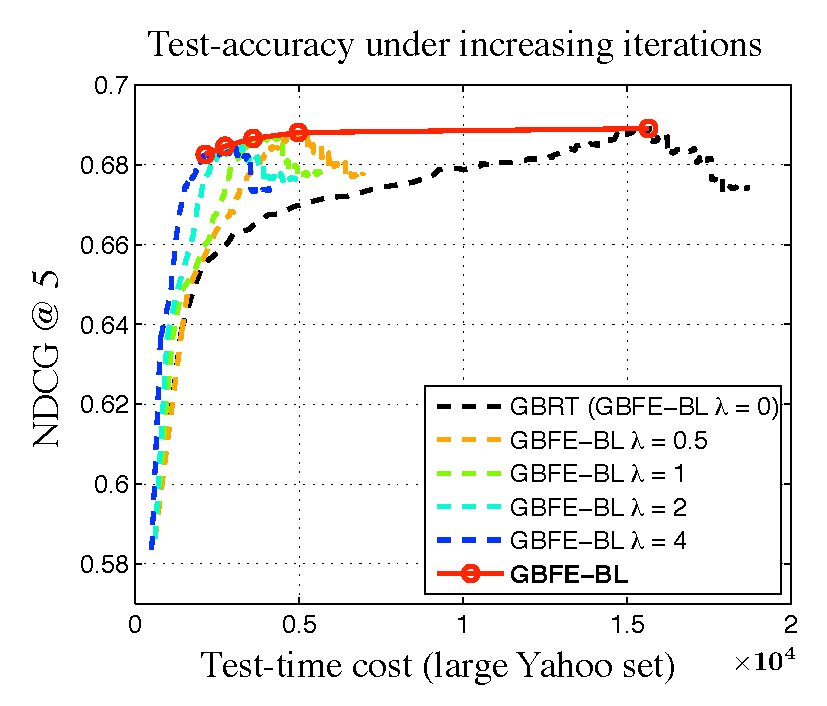
\includegraphics[width = .67\textwidth]{plots/precision_largeset}
}
\vspace{-1.5ex}
\caption{The NDCG@5 and test-time cost performance. The comparison of the original \emph{Gradient Boosted Regression Trees (GBRT) (GBFE-BL with $\lambda = 0$)} and \name{}-BL under various feature-cost/accuracy trade-off settings ($\lambda$) on the full Yahoo set. The dashed lines represent the NDCG@5 as trees are added to each classifier. The red circles indicate the best scoring iteration on the validation data set. \label{fig:precision_largeset}}
\end{figure*}

\textbf{Tuning $\lambda$.}
As shown in Figure \ref{fig:precision_largeset}, different $\lambda$ result in dramatically different performances. Each $\lambda$ corresponds to a feature extraction budget $B_f$, and if the budget is not known during training, selecting $\lambda$ could be problematic. Using a small $\lambda$ guarantees higher scores but may run over budget, using a too large one may cause under-fitting. Since \name{}-BL has a unique property that enables changing $\lambda$ at any iteration, we experiment \name{}-BL with diminishing $\lambda$ to solve the problem of unknown budget during training. Specifically, we set $\lambda$ as a function of the number of iterations $t$, $\lambda = \frac{v}{t}$, where $v$ is a certain initial value. As we gradually add more trees (increasing the number of iterations), the $\lambda$ value decreases. As shown in Figure \ref{fig:lambda}, we evaluate two different initial values ($v \in \{10, 100\}$). Compared to the baselines (fixed $\lambda = 0$ and $\lambda = 1$), the changing ones $\lambda = \frac{v}{t}$ provide smoother curves and can cope with unknown budgets during training. 

\begin{figure*}[t]
\centerline{
% \includegraphics[width = .5\textwidth]{plots/prec-self}
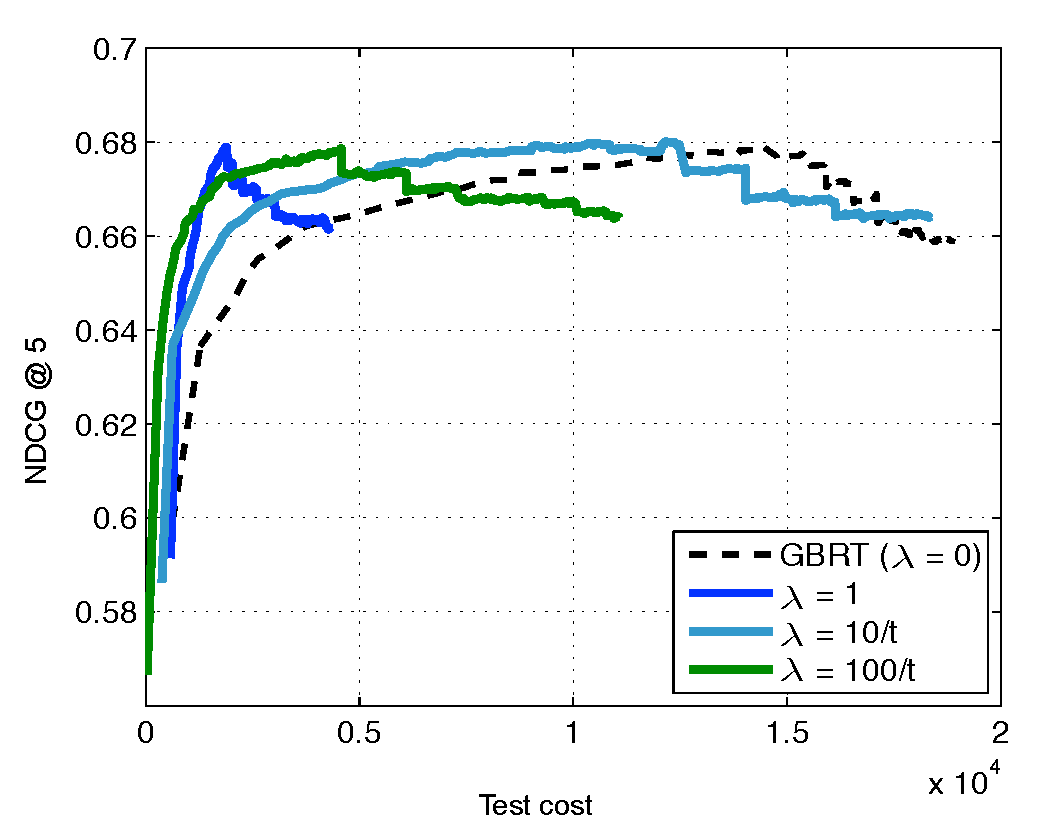
\includegraphics[width = .67\textwidth]{plots/precision_tune}
}
\vspace{-1.5ex}
\caption{The NDCG@5 and the test-time cost of various $\lambda$-settings.
The comparison of the original \emph{Stage-wise regression ($\lambda = 0$)} and \name{}-BL with fixed $\lambda$ and changing $\lambda$ on the full Yahoo set. The dashed lines represent the NDCG@5 as trees are  added to the classifier. Changing $\lambda$ at each iteration provides a smoother curve and can cope with unknown test-time budgets. 
\label{fig:lambda} }
\end{figure*}
 
\textbf{Comparison with prior work. } 
The basic baseline is GBRT, which is equivalent to \name{}-BL with $\lambda = 0$ and $3000$ trees. In addition to GBRT, we also compare against \emph{GBRT feature subsets}, \emph{Early-exit}~\citep{cambazoglu2010early} and \emph{Cronus}~\citep{chen2011}. \emph{GBRT feature subsets} is a natural cost-sensitive extension to GBRT. We first group all features according to their feature extraction cost, and train multiple regular GBRT predictors with gradually more expensive feature groups ($c_f \le 1, 20, 100, 200$). \emph{Early-exit}, proposed by \citet{cambazoglu2010early}, also builds upon GBRT. It first trains trees using regular GBRT, and then removes unpromising documents (with low prediction values) from full evaluation of the boosted ensemble (short-circuiting the sum) during test-time. Since many documents are early-exited, the average test-time cost is reduced. Among all methods of early-exit the authors suggested, we plot the best performing one (Early-exit using proximity threshold). To reduce the average test-time cost, after building all $3000$ trees, we introduce an early-exit every $10$ trees. During test-time, for the $i$th early-exit, we remove all documents that have predicted label value that is $\frac{(300-i)s}{299}$ lower than the fifth-best input. The $s$ is a parameter regulating the pruning aggressiveness, and we generate the performance curve of Early-exit by varying this parameter. The score/cost performance of Early-exit is limited because the cost is dominated by the feature extraction cost and we observe that the first $100$ trees generated by GBRT use almost all features. We also experiment \name{}-BL Early-exit described in Section \ref{sec:early-exit}. To observe the full trend of \name{}-BL Early-exit, we plot its trace as we repeatedly add trees to the predictor and we apply the exact same early-exit procedure described above (remove unpromising documents), and fix the pruning parameter $s = 0.1$.

Since Cronus~\cite{chen2011} does not scale to the full data set, we use the subset of the Yahoo data from~\citet{chen2011} of 141397, 146769, 184968, training, validation and testing points respectively, for comparison in Figure~\ref{fig:precision}. In comparison to Cronus, which requires $O(mn)$ memory, \name{}-BL requires no significant operational memory besides the data and scales easily to millions of data points.

The score and cost trade-off performances of \name{}-BL and competing algorithms are shown in Figure \ref{fig:precision}. To simulate different test-time budgets, we generate the curve of \name{}-BL by varying the feature-cost trade-off parameter $\lambda$. For each setting we choose the iteration that has the best validation NDCG@5 score. The plot demonstrates that without any budget constraints, all algorithms manage to match the highest NDCG@5 score of unconstrained GBRT. However, \name{}-BL maintains a relatively high score at much lower cost and consistently achieves higher scores than Cronus and Early-exit. In fact, \name{}-BL can almost match the ranking accuracy of stage-wise regression with 1/10 of the cost, whereas Cronus reduces the cost only to 1/4 and Early-exit to 1/2. \name{}-BL Early-exit also slightly improves over \name{}-BL.

\begin{figure*}[t]
\centerline{
% \includegraphics[width = .5\textwidth]{plots/prec-self}
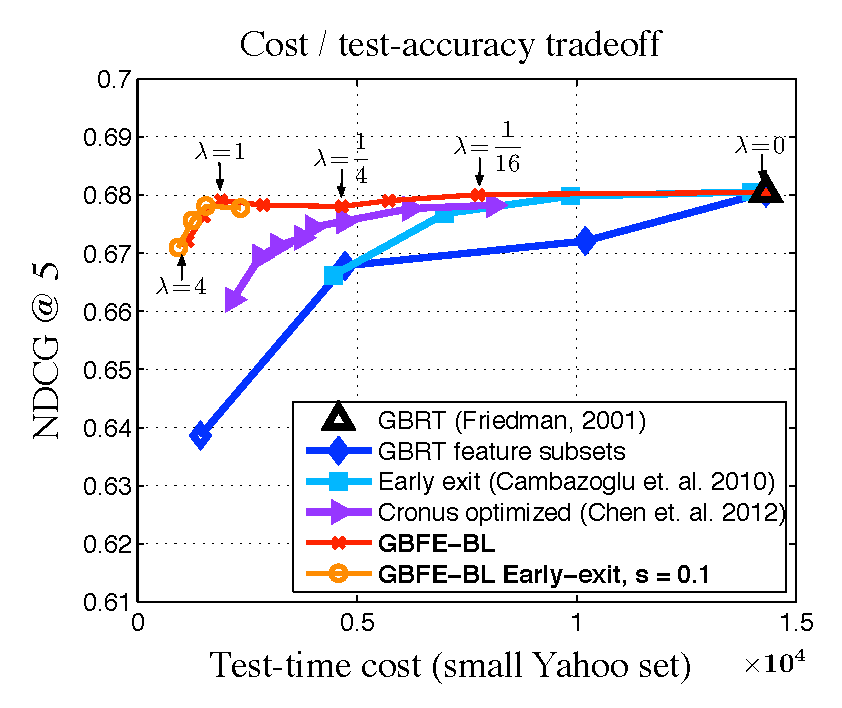
\includegraphics[width = .67\textwidth]{plots/precision_compare}
}
\vspace{-1.5ex}
\caption{Comparisons with prior work on test-time optimized cascades on the small Yahoo set. The cost-efficiency curve of \name{}-BL is consistently above prior work, reducing the cost, at similar ranking accuracy, by a factor of 10.   \label{fig:precision} }
\end{figure*}

\textbf{Feature extraction.}
To investigate the effect the feature-cost trade-off parameter $\lambda$ has on the classifier's feature extraction, Figure~\ref{fig:features} visualizes what type of features are extracted by \name{}-BL as $\lambda$ changes. For this visualization, we group features by cost and show what fraction of features in each group are extracted. The legend in the right indicates the cost of a feature group and the number of features that fall into it (in the parentheses). We plot the feature fraction at the best performing iteration based on the 
validation set. With $\lambda\!=\! 0$,  \name{}-BL does not consider the 
feature cost when building trees, and thus extracts a variety of expensive features. As $\lambda$ increases, it extracts fewer expensive features and re-uses more cheap 
features ($c_\alpha\!=\! 1$). It is interesting to point out that across all different \name{}-BL settings, a few expensive features (cost $\!\ge\!150$) are always extracted within early iterations. This highlights a great advantage of \name{}-BL over some other cascade algorithms~\citep{raykar2010designing}, which learn cascades with pre-assigned feature costs and cannot extract good but expensive features until the very end. 

\begin{figure}[t]
\centerline{
%\includegraphics[width = .5\textwidth]{plots/prec-self}
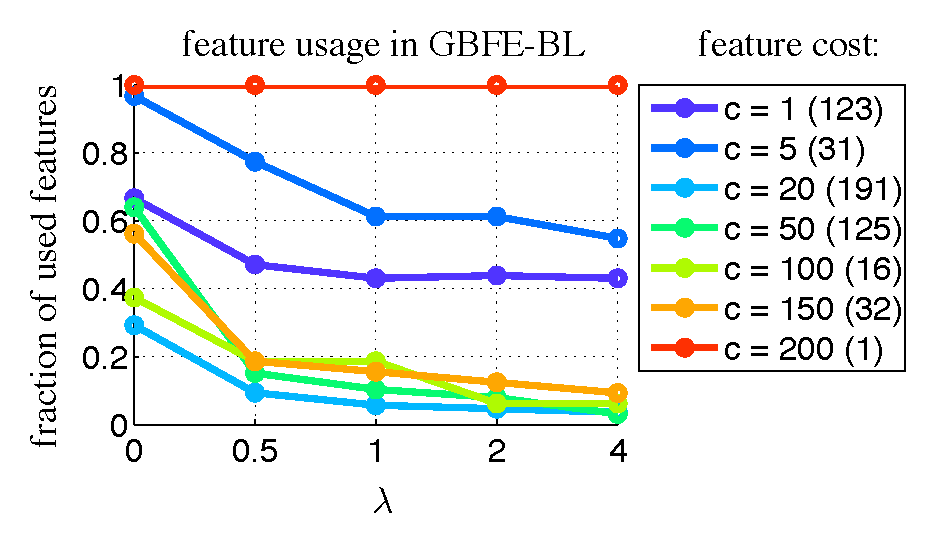
\includegraphics[width = 0.67\textwidth]{plots/features_onegraph}
}
\caption{Features (grouped by cost $c$) used in \name{}-BL with various $\lambda$ (the number of features in each cost group is indicated in parentheses in the legend). 
Most cheap features ($c\!=\!1$) are extracted constantly in different $\lambda$ settings, whereas expensive features ($c\!\geq\! 5$) are extracted more often when $\lambda$ is small. 
The most expensive (and invaluable) feature $c=200$ is always extracted.  
\label{fig:features} }
\end{figure}

\begin{figure}[t]
\centerline{
%\includegraphics[width = .5\textwidth]{plots/prec-self}
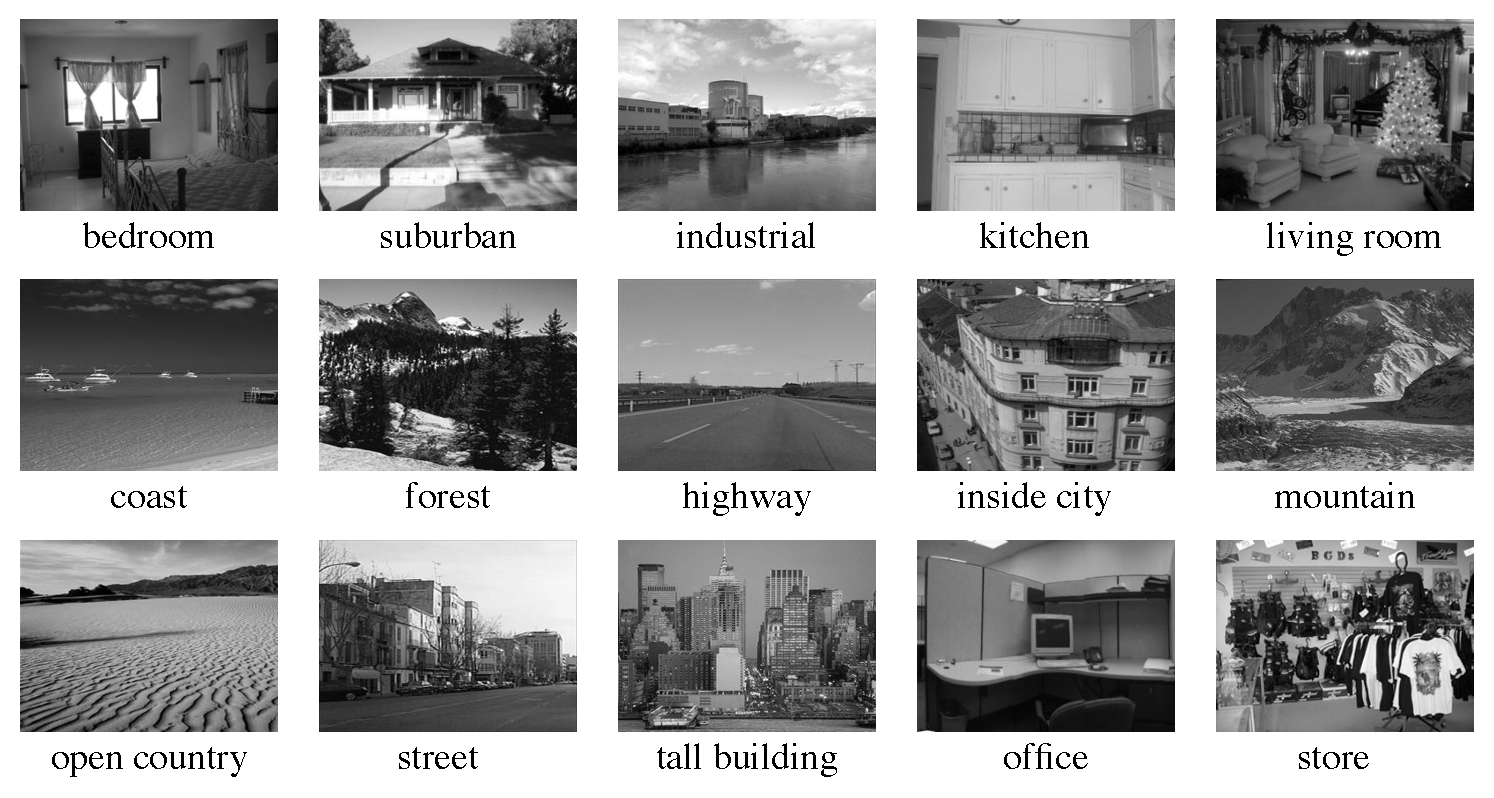
\includegraphics[width = .67\textwidth]{plots/scene15_samples_small}
}
\caption{Sample images of the Scene 15 classification task.\label{fig:sample_images}}
\end{figure}

\begin{figure}[t]
	\vspace{-1.5ex}
\centerline{
%\includegraphics[width = .5\textwidth]{plots/prec-self}
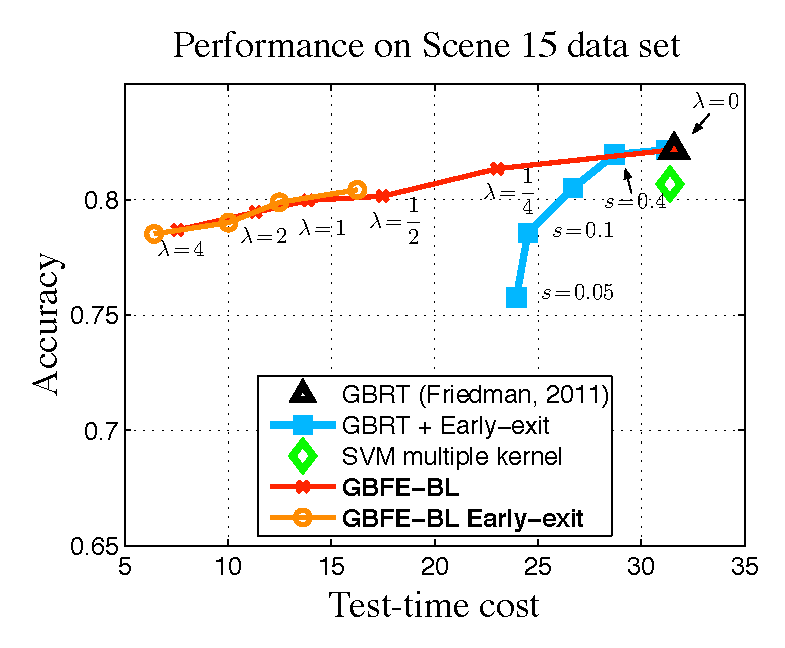
\includegraphics[width = 0.67\textwidth]{plots/scene15_noearly_depth4}
}
\vspace{-1.5ex}
\caption{Accuracy as a function of CPU-cost during test-time. The curve is generated by gradually decreasing $\lambda$. \name{}-BL offers a superior accuracy/cost trade-off and obtains similar accuracy as the SVM with multiple kernels with only half its test-time cost.  \label{fig:scene15}}
\end{figure}

% HERERE
\subsubsection{Scene Recognition} 
The second data set we experiment with is from a very different domain: scene recognition. The Scene-15 data set \citep{lazebnik2006beyond} contains $4485$ images from $15$ different scenes and the task is to classify which scene each image belongs to. Figure~\ref{fig:sample_images} shows example images from each scene category. Following the convention by \citet{lazebnik2006beyond,li2010object}, we subsample 100 images from each class for the training set. From the remaining $2985$ images, we randomly sample $20$ images from each class as a validation set, and use the rest for testing. In total, we have $1500, 300, 2685$ training, validation, and testing images respectively.


We use a diverse set of visual descriptors varying in computation time and accuracy: GIST, spatial HOG, Local Binary Pattern, self-similarity, texton histogram, geometric texton, geometric color, and Object Bank~\citep{li2010object}. Following the convention of \citet{li2010object}, we treat the $177$ object detectors within Object Bank as independent descriptors and in total, we have $7 + 177 = 184$ different visual descriptors. We then split the training set $70/30$ and use the smaller subset to train $15$ one-vs-all kernel SVM classifiers for each descriptor. We use the predictions of the larger subset as our training set features (totaling $d\!=\!184\!\times\! 15\!=\!2760$ features). To train \name{}-BL, we use the multi-class log-loss~\citep{trevor2009elements} and maintain $15$ tree-ensemble classifiers $H^1,\dots,H^{15}$, one for each class. During each iteration, we construct $15$ regression trees (depth 3) and update all classifiers. For a given image, each classifier's (normalized exponential) output represents the probability of this data point belonging to one class. 

Since generating features from different visual descriptors requires different CPU time, the feature extraction cost is naturally defined as the CPU-time required for the computation time for the visual descriptor plus the kernel computation and SVM evaluation. Each visual descriptor is used by $15$ one-vs-all features. The moment any one of these features is used, we set the feature extraction cost of all other features that are based on the same visual descriptor equal to only the SVM evaluation time  (\emph{e.g.} if the first HOG-based feature is used, the cost of all other HOG-based features is reduced to the time required to evaluate the SVM). 

Figure \ref{fig:scene15} demonstrates the performance of various algorithms on the Scene-15 data set. The basic cost-insensitive baselines include \emph{GBRT} \citep{friedman2001greedy} and \emph{SVM} with the averaged kernel of all descriptors. We also apply GBRT with \emph{Early-exit}, where we introduce an early exit every $10$ trees, and during test-time we remove test inputs with the most confident predictions (whose maximum class-likelihood is greater than a threshold $s$). We generate the curve of Early-exit by gradually increasing the value for $s$. The last baseline is multi-class logistic regression~\citep{trevor2009elements} on the original vision features with $l_1$ regularization. We notice that its accuracy never exceeds $0.74$, and therefore we do not plot it. To observe the full range of \name{}-BL, we plot the curve of \name{}-BL by varying its loss/feature-cost trade-off parameter $\lambda$, simulating different budgets. We also include \name{}-BL Early-exit by combining \name{}-BL and Early-exit  together. We use the same procedure as Early-exit described above, but fix the $s = 0.1$. As in experiments on the Yahoo LTR data set, we use the validation set to choose the best number of boosting iterations. We also average over $10$ randomly-generated train/test splits.

While both multiple-kernel SVM and GBRT achieve high accuracy, they are cost-insensitive and extract all features, resulting in a very high cost. Early-exit has very limited improvement due to the inability to select a few expensive but important features in early iterations. \name{}-BL significantly improves over all other baselines and its accuracy drops gently with increasing $\lambda$. \name{}-BL Early-exit slightly improves the cost-accuracy trade-off.

All experiments (on both data sets) were conducted on a desktop with dual 6-core 2.66GHz Intel i7 CPUs. The training time for \name{}-BL requires a comparable amount of time as GBRT (about 80 minutes for the full Yahoo data set and 12 minutes for Scene-15.)


\subsection{Feature selection}

\begin{figure}[t!!!]
\centerline{
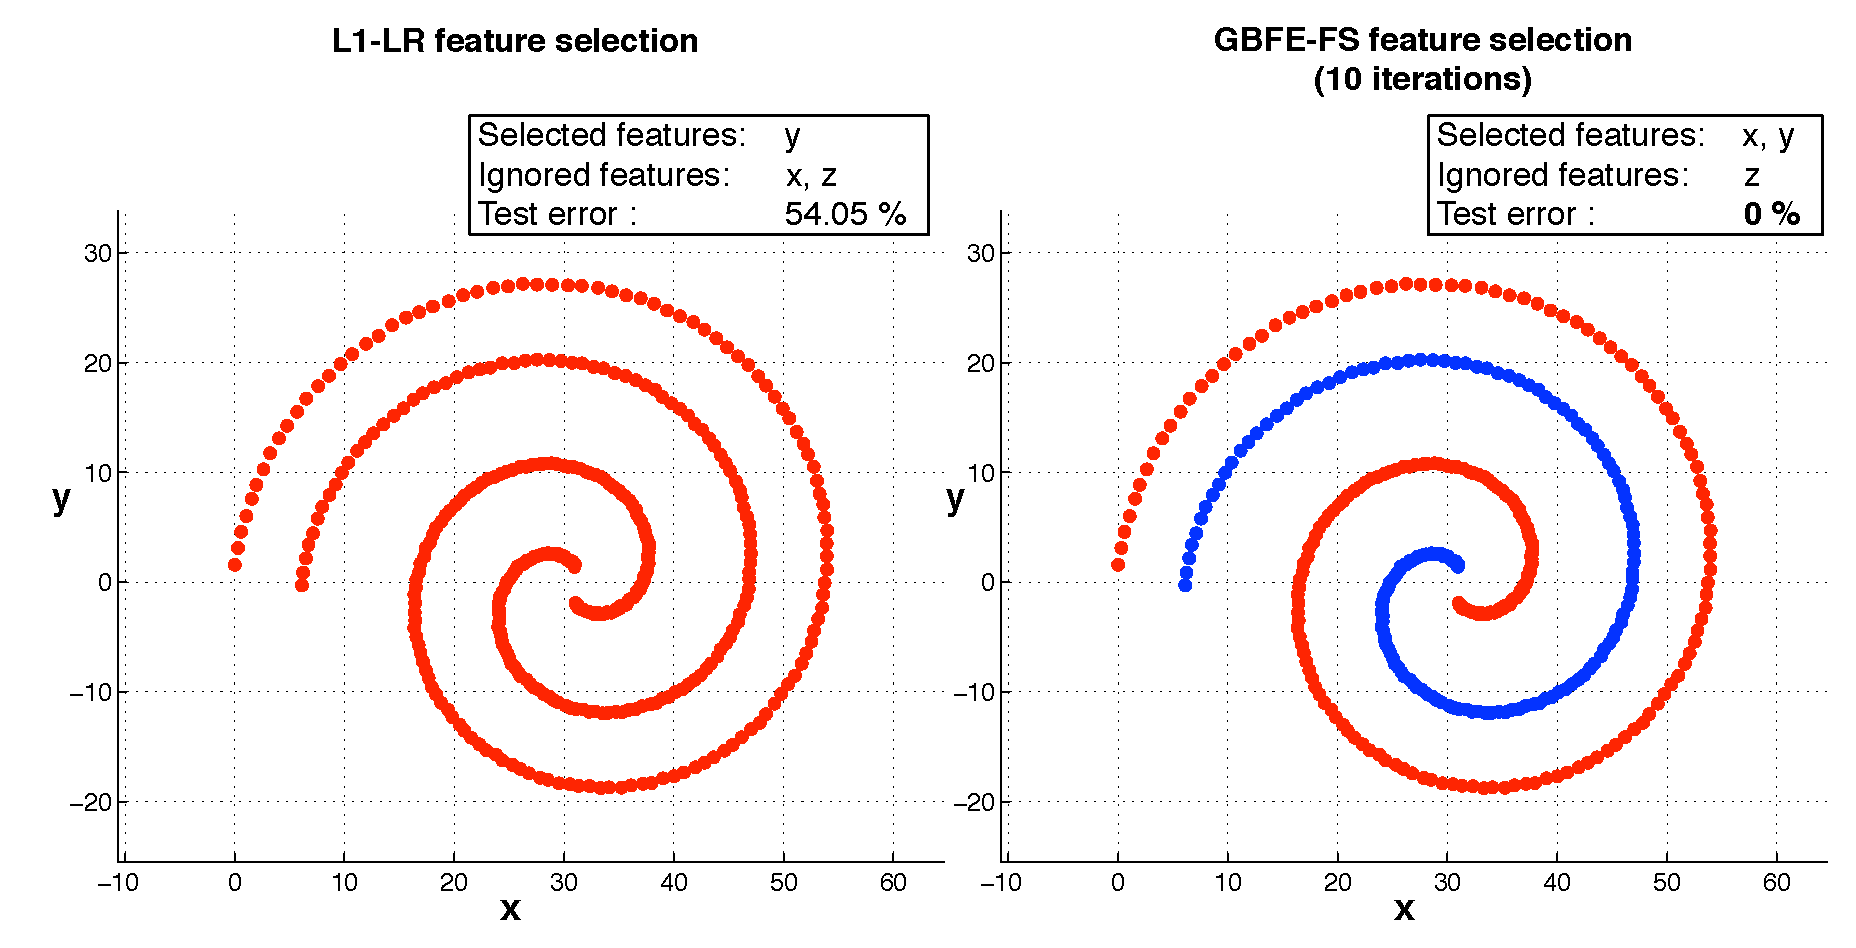
\includegraphics[width = .9\textwidth]{plots/simul}
}
\caption{Feature selection and classification performance on a simulation data set. \name{}-FS clearly outperforms the $l_1$-regularized logistic regression as it successfully captures the non-linear relations between labels and features.}
\label{fig:res_simul}
\end{figure}

In this section, we experiment with the feature selection extension of \name{}, \name{}-FS. We first evaluate it on a synthetic data set to demonstrates its unique properties, and then experiment on a bioinformatics application to evaluate its capability of selecting features with known sparsity patterns. We further compare \name{}-FS with several current state-of-the-art feature selection methods on benchmark data sets. 

\subsubsection{Synthetic data}
The synthetic data is shown in Figure \ref{fig:res_simul}. The data set is a binary classification problem and contains three features, $x$, $y$ and $z$ (where $z$ is a linear combination of $x$ and $y$, and is therefore redundant). While the data is not linearly separable in either two or three dimensions, a good \emph{non-linear} classifier should easily separate the data only based on $x$ and $y$. %The $z$ feature is a linear combination of $x$ and $y$ and is redundant. 
We randomly select $90\%$ of the instances for training and the rest for testing. 

The first baseline is \emph{$l_1$-regularized logistic regression} (L1-LR) \cite{lee2006efficient,park2007l1}. L1-LR selects features by applying an $l_1$-norm on the weight vector to produce a sparse solution. The regularization constant was set on a hold-out set. While L1-LR feature selection successfully detects the redundant feature $z$, it fails to identify a non-linear combination of $x$ and $y$ that renders good classification rates, and only selects one feature $y$. As a result, its classification error rate is very high ($54.05\%$). In contrast, \name{}-FS not only identifies the redundant feature $z$, but also detects that labels are related by a non-linear combination of $x,y$. It successfully separates the classes by selecting both $x$ and $y$ features, achieving a $0\%$ test error rate. 

\begin{figure}[t!!!]
\centerline{
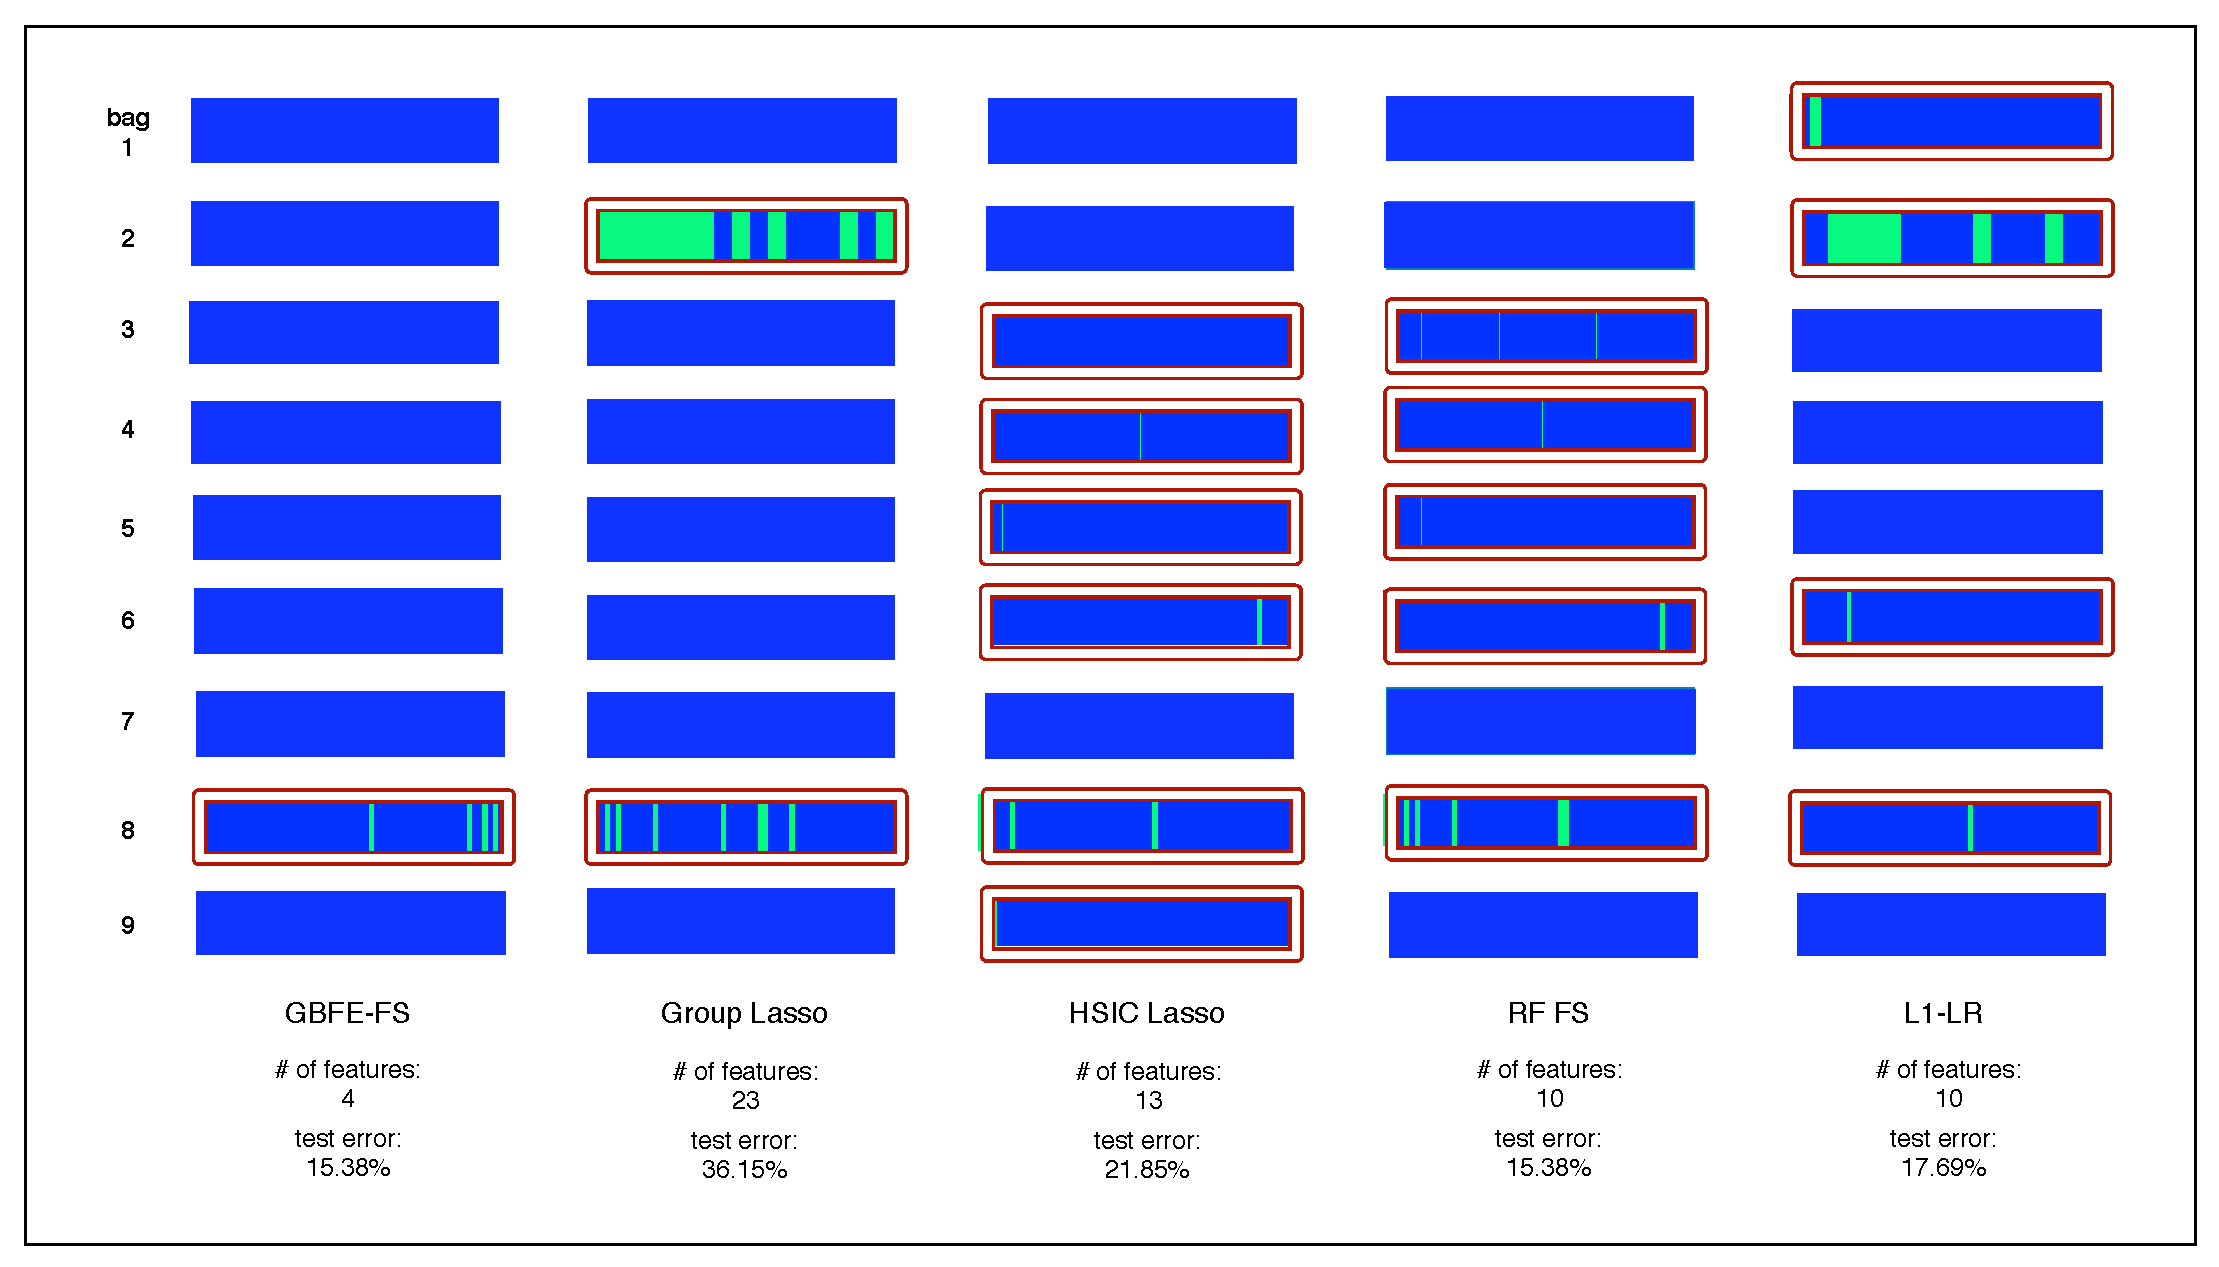
\includegraphics[width = 1\textwidth]{plots/biology_horizental}
}
% \vspace{-8pt}
\caption{Feature selection on a structured feature data set. Selected features are colored in green, and unselected are in blue. The bag is highlighted with a red/white box if at least one of its features is selected. (Some bags may require zooming in to make the selected features visible.)}
% \vspace{-10pt}
\label{fig:bag}
\end{figure}

\subsubsection{Structured feature selection}
In many real-world applications prior feature sparsity information may be provided. For example in bioinformatics or neuroscience if a classifier uses some features (such as genes or brain regions) to make predictions, it has to be biologically and neurologically explainable.

Since \name{}-FS can naturally incorporate pre-specified feature structures, we evaluate \name{}-FS for structured feature selection on the Colon data set\footnote{Available at Princeton University gene expression project: http://microarray.princeton.edu/oncology/}. In this new biology data set, $40$ tumor and $22$ normal colon tissues for $6500$ human genes are measured using Affymetrix gene chips. Among $6500$ genes, $2000$ are selected as they have the highest minimal intensity across the samples \citep{alon1999broad}. \citet{ma2007supervised} further analyze these genes and cluster them into $9$ clusters/bags according to their biological meaning. The task is to classify whether a tissue is normal or tumorous, and which cluster of genes contribute to this. We randomly split the $62$ tissues into $80/20$ training and testing datasets, repeated over $10$ random splits.
We use the feature-bag cost function $\phi_s$ mentioned in Section~\ref{sec:structure} to incorporate this side-information (setting the cost of all features in a bag to \emph{zero} once the first feature is extracted). Feature selection without considering this bag information not only performs and 
generalizes poorly, but are also difficult to interpret and justify. 

Figure \ref{fig:bag} shows the selected features from one random split and classification error rates averaged over $10$ splits. Selected features are colored in green, and unselected ones are in blue. A bag is highlighted with a red/white box if at least one of its features is selected. As for baselines, we include \emph{$l_1$-regularized logistic regression (L1-LR)}~\citep{lee2006efficient,park2007l1}, \emph{Random Forest Feature Selection (RF FS)}, \citep{trevor2009elements}, \emph{HSIC Lasso}~\citep{yamada2012high} and \emph{Group Lasso with logistic regression (Group Lasso)}~\citep{meier2008group}. 

Shown in Figure \ref{fig:bag}, \name{}-FS successfully incorporates the bag structures and focusses on selecting features from one specific bag. It selects features exclusively from bag $8$ throughout (highlighted with a red/white box in the figure). This allows the selected features to reveal the association between diseases and gene clusters/bags. Similarly, Group Lasso can also incorporate structure information. However, different from \name{}-FS, the $l_2$ regularization of Group lasso has side effects on feature weights, and thus results in a much higher error rate $36.15\%$. The rest of the algorithms: L1-LR, RF FS, and HSIC Lasso do not take bag information into consideration, and select scattered features from various bags. In terms of classification error rates, \name{}-FS matches the best performing RF FS at $15.38\%$, and out-performs L1-LR and HSIC lasso, which achieve $17.69\%$ and $21.85\%$ respectively. 

% Our explanation why \name{} can be accurate with features from only a single bag is two-fold: 1. it is indeed the case that the genes in bag $8$ are very predictive for testing if tissue is malignant or benign (a result that may be of high biological value); 2. \name{} does not penalize further feature extraction inside bag $8$ and can build a more accurate classifier than other methods, which keep penalizing all feature extractions.


\begin{table*}[t]
	\begin{center}
\begin{tabular}{|l||c|c|c|c|c|c|c|}
  \hline
  \bf{data set} & pcmac & uspst & spam & isolet & mnist3vs8 & adult & kddcup99\\
  \hline \hline
  \bf{\#training} & 1555 & 1606 & 3681 & 6238 & 11982 & 32562 & 4898431 \\ 
  \hline
  \bf{\#testing} & 388 & 401 & 920 & 1559 & 1984 & 16282 & 311029\\
  \hline 
  \bf{\#features} & 3289 & 256 & 57 & 617 & 784 & 123 & 122 \\
  \hline
\end{tabular}
	\caption{Dataset statistics. Datasets are ordered by the number of training instances.}  \label{table:datasets}
	\end{center}
\end{table*}

\subsubsection{Benchmark data sets}
In this section, we compare \name{}-FS against the current state-of-the-art in feature selection on several benchmark data sets.

\textbf{Data sets.}
Table \ref{table:datasets} lists dataset statistics ordered by increasing numbers of training instances. In this paper, we focus on a new scenario where the number of instances is much greater than the number of dimensions ($n \gg p$). While \name{}-FS can naturally extend to multi-class or regression settings, for simplicity, we convert all problems to binary classification, either by selecting the two classes that are most easily confused or (if those are not known) by grouping labels into two sets.

\textbf{Baselines.} 
The first baseline we include is \emph{$l_1$-regularized logistic regression (L1-LR)}~\citep{lee2006efficient,park2007l1}. To observe the performance of the full feature selection spectrum, we vary the regularization parameter to select different numbers of features.

We also include \emph{Random Forest Feature Selection (RF FS)}~\citep{trevor2009elements}. Similar to \name{}-FS, RF FS is a non-linear feature selection algorithm. It trains a Random Forest by building many full trees using subsets of features. It then ranks all features according to their cumulative contribution to the impurity improvement in each split, in each tree. Features with larger impurity improvement are considered more important. Throughout we run RF FS with $2000$ trees and a maximum number of $20$ instances per leaf node. After training all $2000$ trees, we rank all features. Starting from the most important features, we gradually select less important features and repeatedly re-train Random Forests with only selected features. We stop once we include all features.

The next baseline is \emph{Minimum Redundancy Maximum Relevance (mRMR)}~\citep{peng2005feature}. mRMR selects features based on their mutual information with the labels of each instance. We gradually increase the desired number of features using mRMR until we include all features. Since mRMR is not a classifier, we train an RBF kernel SVM using features selected by mRMR for classification. We tune the hyper-parameters of the SVM on $5$ different random $80/20$ splits of the training data. 

The last competing algorithm is HSIC Lasso~\citep{yamada2012high}, which is a convex extension to Greedy HSIC~\citep{song2012feature}. HSIC Lasso builds a kernel matrix for each feature, and linearly combines them to best match an ideal kernel generated from the labels. To perform feature selection, it applies an $l_1$-norm penalty on the coefficients of each kernel matrix. We evaluate a wide range of $l_1$ regularization parameters to plot the full feature selection range. Once features are selected, we train a kernel SVM with the selected features to perform classification. Similar to the mRMR experiment, we use cross-validation to select hyper-parameters and average over $5$ runs.

To evaluate \name{}-FS, we first $80/20$ split the training data into a training and validation set, and use the validation set to cross-validate two hyper-parameters (the depth of the regression trees and the number of iterations). Throughout, we fix the learning rate $\eta = 0.1$ as the model is fairly insensitive to this choice. To observe the full range of feature selection performance, we evaluate \name{}-FS with $10$ different trade-off parameters $\lambda$ (i.e., $\lambda = \{2^{-3},2^{-2},2^{-1},2^0,2^1,2^2,2^{3},2^{5},2^7,2^9\}$).

\begin{figure*}[t!!!]
\centerline{
% \includegraphics[width = 0.9\textwidth]{plots/results}
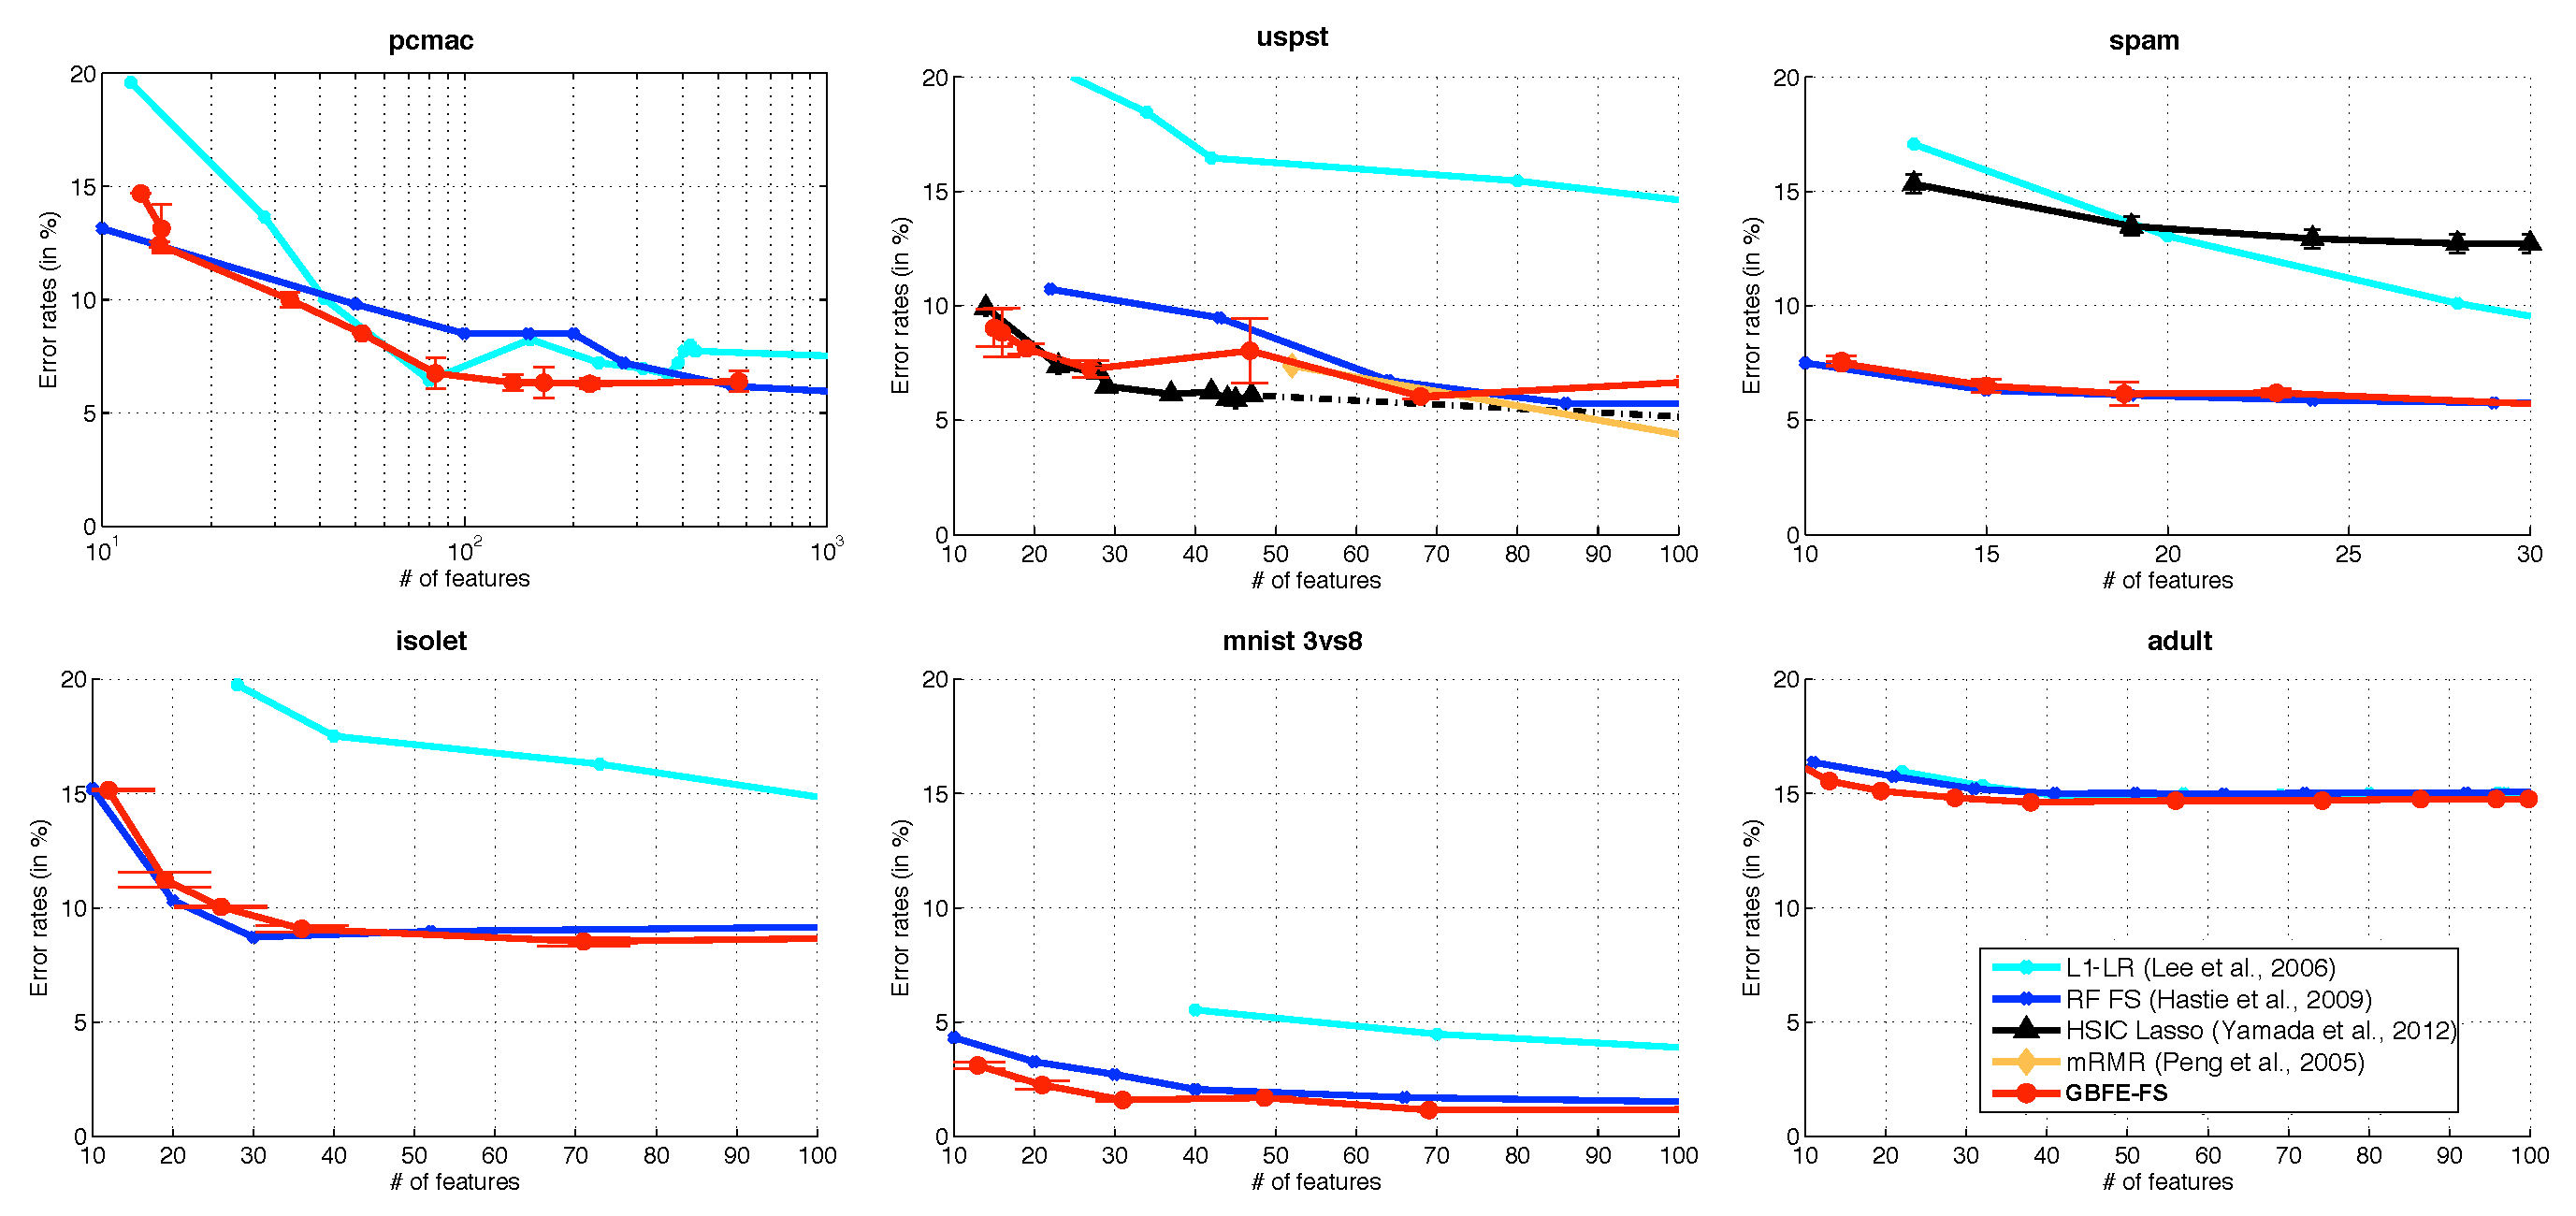
\includegraphics[width = 1.05\textwidth]{plots/results_071_100}
}
\caption{Classification error rates (in \%) vs.\ feature selection performance for different algorithms on small to medium sized datasets.}
\label{fig:results}
\end{figure*}

\textbf{Benchmark error rates.}
The performance of different algorithms on small and medium size datasets is shown in Figure \ref{fig:results}. We show the error rate levels up to 100 features except for \emph{spam} which only has $p=57$ dimensions and \emph{pcmac}, which is higher dimensional ($p=3289$). 

We observe that L1-LR, RF FS, and \name{}-FS can easily scale to all data sets. Both RF FS and \name{}-FS clearly out-perform L1-LR in accuracy on data sets because of their ability to capture non-linear feature-label correlations. HSIC Lasso and mRMR are very sensitive to the data size (both the number of training instances and the number of features), and only scale to small data sets. On small data sets where they scale, \name{}-FS still out-performs HSIC Lasso on one data set and matches mRMR. Compared to RF FS, \name{}-FS either out-performs or matches its performance on all data sets. However, one advantage of \name{}-FS is that it is a one step approach, selecting features and learning a classifier at the same time. In contrast, RF FS requires re-training a classifier after feature selection.

\begin{figure}[t!!!]
\centerline{
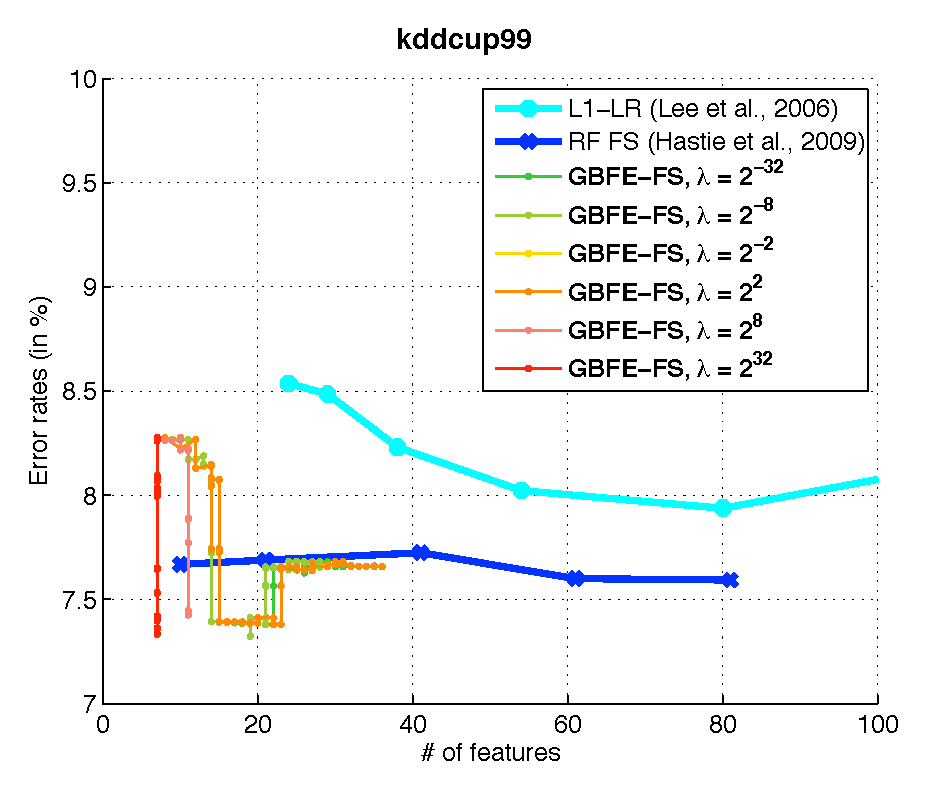
\includegraphics[width = 0.67\textwidth]{plots/largeset_071}
}
\caption{Feature selection and classification error rates (in \%) for different algorithms on the large \emph{kddcup} data set.}
% \vspace{-15pt}
\label{fig:largeset}
\end{figure}

\textbf{Massive data.}
The last data set in Table~\ref{table:datasets} (\emph{kddcup99}) contains close to 5 million training instances. Performing feature selection on such a massive dataset can be very time-consuming. We limit \name{}-FS to $500$ trees with the default hyper-parameters of tree depth $4$. Training a regular Random Forest with all default hyper-parameters would take more than a week. Therefore, we limit the number of trees to $100$ and the maximum number of instances per leaf node to $500$. As shown in Figure \ref{fig:largeset}, we plot the whole traces of \name{}-FS as we gradually add trees. Different traces are shown for different feature sparsity regularizer values $\lambda$. \name{}-FS obtains lower classification error rates than both RF FS and L1-LR when fewer features are selected. (Note that due to the extremely large data set size, even improvements $<1\%$ are considered significant).

\begin{figure}[t!!!]
\centerline{
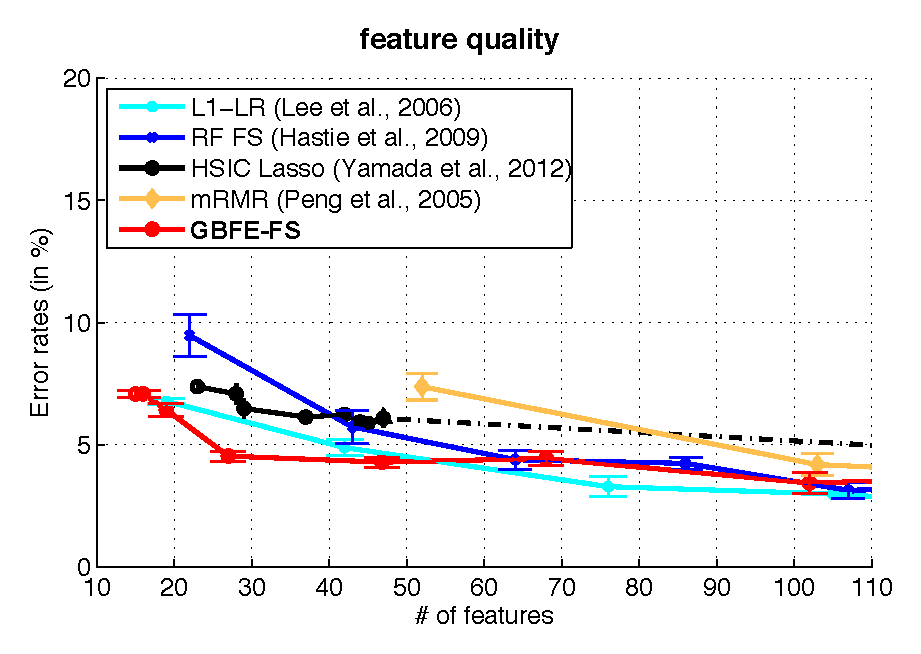
\includegraphics[width = .75\textwidth]{plots/feature_quality}
}
\caption{Error rates (in \%) of an RBF-kernel SVM trained on various feature subsets obtained with different feature selection algorithms.}
% \vspace{-18pt}
\label{fig:quality}
\end{figure}

\textbf{Feature quality.}
Since not all competing algorithms combine feature selection with classification, we separate these two tasks to further evaluate the feature selection quality of each algorithm. We run all algorithms on the smallest data set (\emph{uspst}) to select features, and then train an SVM with an RBF kernel. Figure \ref{fig:quality} shows the test error rate as a function of the number of selected features. When only a few features are selected, \name{}-FS obtains the lowest error rate. As more features are selected. all algorithms converge to similar test error. Note that the linear feature selection algorithm L1-LR out-performs most non-linear algorithms. This suggests that the \emph{uspst} digits dataset requires a non-linear classifier for classification but not for feature selection.

% \textbf{$d\gg n$ scenario.}
% While \name{} focusses on the scenario where the number of inputs is much larger than the number of features ($n\gg d$), we also evaluate \name{} on a traditional feature selection benchmark data set SMK-CAN-187~\cite{spira2007airway}, which is publicly available from~\cite{zhao2010advancing}. This binary classification data set contains $187$ inputs and $19,993$ features. We randomly select $80\%$ percent of inputs as training and $20\%$ as testing and we average over $5$ runs. Figure~\ref{fig:high_dims} shows the comparison results. \name{} out-performs $l_1$ regularized logistic regression (L1-LR), HSIC-Lasso and Random Forest feature selection (RF FS) algorithms.



% \begin{figure}[t!!!]
% \centerline{
% \includegraphics[width = 1.1\columnwidth]{plots/timing}
% }
% \caption{Training run-time for different algorithms on small to medium sizes datasets.}
% \label{fig:timing}
% \end{figure}

\subsubsection{Analysis of variance.}

\subsubsection{Computation time and complexity.} 
The fastest method so far is the linear algorithm, L1-LR. On the other hand, non-linear algorithms mRMR and HSIC Lasso are much more time consuming because their methods involve either expensive mutual information or kernel matrix computations, which scale $O(d^2)$ or $O(n^2)$. RF FS is in the middle. It builds full trees, requiring a time complexity of $O\Big(\sqrt{d}n\log(n)\Big)$ per tree, where the $\sqrt{d}$ comes from the fact that Random Forests always use a square root of number of features every time it builds a tree. 

In contrast, \name{}-FS only builds limited depth trees (depth = 4,5), and the computation time complexity is $O(dn)$. Empirically, we observe that RF FS and \name{}-FS are comparable in speed but \name{}-FS is significantly faster on data sets with many instances (large $n$). The training time ranges from several seconds to minutes on small data sets and to approximately one hour on the larger data set \emph{kddcup99} (this is the case for RF FS only if trained with only $500$ trees and large leaf sizes). 


% Unsurprisingly, the fastest method by far is  the only linear algorithm, $l_1$ regularized logistic regression.
% Both mRMR and HSIC Lasso take significantly more time than Random Forest and \name{} because they involve either mutual information or kernel matrix computation, which scales $O(d^2)$ or $O(n^2)$. Random Forest builds full trees, requiring a time complexity of $O(\sqrt{d}n\log(n)$ per tree. The  dependency on $\sqrt{d}$ is slightly misleading, as the number of trees required for Random Forests is also depended on the number of features and scales $O(\sqrt{d})$ itself.
% In contrast, \name{} only builds limited depth (depth = $4,5$) trees, and the computation time complexity is  $O(dn)$. The number of iterations $T$ is independent of the number of input features $d$ and only a function of how many features are desired to be selected.
% Empirically, we observe that the two algorithms are comparable in speed but \name{} is significantly faster on data sets with many instances (large $n$). The training time ranged from several seconds to minutes on the small data sets to about one hour on the large data  set \emph{kddcup99} (if Random Forest is trained with only 500 trees and large leaf sizes).
% Admittedly, the empirical comparison of training time is slightly problematic because our Random Forest implementation is based on highly optimized C++ code, whereas \name{} is implemented in Matlab\texttrademark. We expect that \name{} could be made significantly faster if implemented in faster programming languages (\emph{e.g.} C++) with the incorporation of known parallelization techniques for limited depth trees~\cite{tyree2011parallel}.
%Comparing training time between \name{} and Random Forests is difficult for two reasons: For Random Forest we used a highly optimized C++ optimization, whereas \name{} was implemented in Matlab\texttrademark. Further, both algorithms can be run for any number of trees, thus trading off time complexity for feature quality. Overall, Random Forests and \name{} require about the same amount of time

%Therefore, on small data sets (\emph{uspst, spam}), \name{} is $3$X faster than Random Forest, and on medium size data sets, \name{} is faster by a factor of $5$ to $10$. For the large data set \emph{kddcup99}, \name{} takes $2.2$ hours to train $500$ trees, and Random Forest takes $6.2$ hours to train $100$ trees with minimum $500$ instances in leaf nodes, which performs worse than \name{}.














\section{Related Work}
\label{sec:related}
%!TEX root=gm_jmlr.tex

In this section, we present prior work from two domains: budgeted learning and feature selection. 

\subsection{Prior work in budgeted learning}
Previous work in budgeted learning appears in many different applications. The most prominent was proposed by \citet{viola2004robust}. They greedily trained a cascade of classifiers with Adaboost~\citep{schapire1999brief} for fast object recognition.  \citet{cambazoglu2010early} then introduced the cascade framework to the setting of web-search ranking. Their algorithm is based on regular stage-wise regression, and during testing, they remove unpromising instances early-on using early-exits. \citet{Lefakis2010} and \citet{dundar2007joint} further extended the cascade framework by proposing soft-cascades, which re-weight inputs based on their probability of passing all stages. Very different from \name{}-BL, they do not consider the feature extraction cost explicitly during training and their algorithms are restricted to binary classification problems. 

To consider feature extraction cost, \citet{GaoKoller11} proposed to dynamically extract features during test-time. \citet{raykar2010designing} learn cost-sensitive classifier cascades by explicitly considering feature cost. They group features by their costs and restrict classifiers at each stage to only use small  feature subsets. \citet{pujara2011using} suggested the use of sampling to derive a cascade of classifiers with increasing cost for email spam filtering.  Most recently, \citet{chen2011} introduced Cronus, which explicitly considers the feature extraction cost during training and constructs a cascade to encourage removal of unpromising data points early-on. While effective, these algorithms require significant time to train. In contrast, \name{}-BL is a natural variant of fast stage-wise regression, and can operate in both regression and multi-class classification scenarios. 

% We pursue a very different (orthogonal) approach and do not optimize the cascade stages globally. Instead, we strictly incorporate the feature cost into the weak learners. Moreover, as our algorithm is a variant of stage-wise regression, it can operate naturally in both regression and multi-class classification scenarios. (Simultaneous with this publication,~\citet{grubb2012} also proposed a complementary approach to incorporate feature cost into gradient boosting.)

\subsection{Prior work in feature selection}
One of the most widely used feature selection algorithms is Lasso~\citep{tibshirani1996regression}. It minimizes the squared loss with $l_1$ regularization on the coefficient vector, which encourages sparse solutions.  Although scalable to very large data sets, Lasso models only linear correlations between features and labels and cannot discover non-linear feature dependencies. 

\citet{peng2005feature} proposed the Minimum Redundancy Maximum Relevance (mRMR) algorithm, which select features according to their mutual information with instance labels. Their objective function also penalizes selecting redundant features. However, computing mutual information is intractable when the training size is large. \citet{yamada2012high} introduced HSIC Lasso. Their algorithm introduces non-linearity by using kernel functions and performs feature selection by enforcing an $l_1$-norm on the coefficients of kernel matrices. The algorithm requires constructing kernel matrices for all features, thus its time and memory complexity scale quadratically with the dataset size. Moreover, both algorithms separate feature selection and classification, and require additional time and computation for training classifiers using the selected features.

Several other works avoid expensive kernel computation while maintaining non-linearity.  Grafting~\citep{perkins2003grafting} combines $l_1$ and $l_0$ regularization with a non-linear classifier based on a non-convex variant of the multi-layer perceptron. Feature selection for ranking using boosted trees~\citep{pan2009feature} and selects the top features with the highest relative importance scores. \cite{tuv2009feature} and \cite{trevor2009elements} use random forests to select features based on their frequency of use in tree splits. These algorithms may be seen as complimentary to the models proposed in this work. 
%by ranking all features from the forest by their accumulated impurity improvement in all splits. \cite{tuv2009feature} introduces artificial features and masking scores to Random Forest feature selection to further remove irrelevant features. 
% Finally, while not a feature selection method, \cite{greedymiser} employ Gradient Boosted Trees to learn cascades of classifiers to reduce test-time cost by incorporating feature extraction budgets into the classifier optimization. 

\section{Conclusions}
\label{sec:conclude}
%!TEX root=gm_jmlr.tex 

\label{sec:conclusion}
In this paper, we comprehensively demonstrate the usefulness of gradient boosted regression trees (GBRT) for feature selection applications. We derive a novel algorithm that simultaneously performs feature selection and classification for widely differing settings. First, we show that if feature extraction requires a cost (e.g., CPU-time, monetary, patient discomfort) we can directly incorporate this cost into the gradient boosted optimization procedure of GBRT. Second, if we have prior knowledge that features are structured (e.g., for bio-informatics) we can seamlessly encode it in a regularization term for learning each tree. The power of a unified boosting procedure for (cost-sensitive) feature selection and classification is clearly demonstrated on multiple budgeted and real-world genomic datasets. In nearly all settings, \name{}-BL and \name{}-FS outperform the state-of-the-art.

As more and more practitioners look to machine learning for (a) efficient data-driven alternatives to intricate heuristics and (b) interpretable classification algorithms, the problems of cost-sensitive learning and feature selection are of increasing significance. Alongside the gradient boosted models proposed here, there are many directions for future work. Adapting GBRT-based approaches to the setting of \emph{anytime learning} \cite{zilberstein1996using}, in which a fixed cost budget for classification is unknown prior to test-time, would be worth further investigating, alongside the work of \citet{grubbspeedboost}. As well, it may be fruitful to consider ways to encode probabilistic feature structure into these models. We believe the models proposed here are a strong contribution towards addressing the requirements of practitioners for machine learning.

% Acknowledgements should go at the end, before appendices and references

% \acks{We would like to acknowledge support for this project
% from the National Science Foundation (NSF grant IIS-9988642)
% and the Multidisciplinary Research Program of the Department
% of Defense (MURI N00014-00-1-0637). }

% Manual newpage inserted to improve layout of sample file - not
% needed in general before appendices/bibliography.

\newpage

\appendix
%\section*{Appendix A.}
%\label{app:theorem}

\vskip 0.1in
\bibliography{gm_jmlr}

\end{document}
